%% Copernicus Publications Manuscript Preparation Template for LaTeX Submissions
%% ---------------------------------
%% This template should be used for copernicus.cls
%% The class file and some style files are bundled in the Copernicus Latex Package which can be downloaded from the different journal webpages.
%% For further assistance please contact the Copernicus Publications at: publications@copernicus.org
%% http://publications.copernicus.org


%% Please use the following documentclass and Journal Abbreviations for Discussion Papers and Final Revised Papers.


%% 2-Column Papers and Discussion Papers
\documentclass[esd, manuscript]{copernicus}



%% Journal Abbreviations (Please use the same for Discussion Papers and Final Revised Papers)

% Archives Animal Breeding (aab)
% Atmospheric Chemistry and Physics (acp)
% Advances in Geosciences (adgeo)
% Advances in Statistical Climatology, Meteorology and Oceanography (ascmo)
% Annales Geophysicae (angeo)
% ASTRA Proceedings (ap)
% Atmospheric Measurement Techniques (amt)
% Advances in Radio Science (ars)
% Advances in Science and Research (asr)
% Biogeosciences (bg)
% Climate of the Past (cp)
% Drinking Water Engineering and Science (dwes)
% Earth System Dynamics (esd)
% Earth Surface Dynamics (esurf)
% Earth System Science Data (essd)
% Fossil Record (fr)
% Geographica Helvetica (gh)
% Geoscientific Instrumentation, Methods and Data Systems (gi)
% Geoscientific Model Development (gmd)
% Geothermal Energy Science (gtes)
% Hydrology and Earth System Sciences (hess)
% History of Geo- and Space Sciences (hgss)
% Journal of Sensors and Sensor Systems (jsss)
% Mechanical Sciences (ms)
% Natural Hazards and Earth System Sciences (nhess)
% Nonlinear Processes in Geophysics (npg)
% Ocean Science (os)
% Proceedings of the International Association of Hydrological Sciences (piahs)
% Primate Biology (pb)
% Scientific Drilling (sd)
% SOIL (soil)
% Solid Earth (se)
% The Cryosphere (tc)
% Web Ecology (we)
% Wind Energy Science (wes)


%% \usepackage commands included in the copernicus.cls:
%\usepackage[german, english]{babel}
%\usepackage{tabularx}
%\usepackage{cancel}
%\usepackage{multirow}
%\usepackage{supertabular}
%\usepackage{algorithmic}
%\usepackage{algorithm}
%\usepackage{amsthm}
%\usepackage{float}
%\usepackage{subfig}
%\usepackage{rotating}


\begin{document}

\title{TEXT}


% \Author[affil]{given_name}{surname}

\Author[1]{Doug}{McNeall}
\Author[2]{Jonny}{Williams}
\Author[1]{Ben}{Booth}
\Author[1]{Richard}{Betts}
\Author[3]{Peter}{Challenor}
\Author[1]{Andrew}{Wiltshire}
\Author[1]{David}{Sexton}


\affil[1]{Met Office Hadley Centre, FitzRoy Road, Exeter, EX1 3PB UK}
\affil[2]{NIWA, New Zealand}
\affil[3]{University of Exeter, North Park Road, Exeter EX4 4QE UK}

%% The [] brackets identify the author with the corresponding affiliation. 1, 2, 3, etc. should be inserted.



\runningtitle{TEXT}

\runningauthor{TEXT}

\correspondence{Doug McNeall (doug.mcneall@metoffice.gov.uk)}



\received{}
\pubdiscuss{} %% only important for two-stage journals
\revised{}
\accepted{}
\published{}

%% These dates will be inserted by Copernicus Publications during the typesetting process.


\firstpage{1}

\maketitle



\begin{abstract}
We use observations of forest fraction to constrain carbon cycle and land surface input parameters of the reduced resolution global climate model, FAMOUS. Using a history matching approach along with a computationally cheap statistical proxy (emulator) of the climate model, we compare an ensemble of simulations of forest fraction with observations, and rule out parameter settings where the forests are poorly simulated. 

Regions of parameter space where FAMOUS best simulates the Amazon forest fraction are incompatible with the regions where FAMOUS best simulates other forests. Previous studies using climate models have used similar methods to find previously untried candidate input parameter sets that remove what was assumed an underlying structural error. We offer a counter example, arguing that we have found a true structural discrepancy. This has implications for the calibration of FAMOUS: using observations of different forest regions to calibrate the model leads to very different conclusions about the best values, the corresponding uncertainty of input parameters, and potentially, predictions of future forest cover. Dealing with this structural discrepancy is vital when choosing a set of "best" parameters for the land surface - failure to do so could lead to poor parameter selection.

We characterise the structural model discrepancy, and explore the consequences of ignoring it in a history matching exercise. We perform a sensitivity analysis to find the parameters most responsible for simulator error and therefore most promising for tuning.  We use the emulator to simulate the forest fraction at the best set of parameters implied by matching the model to the Amazon, and to other major forests in turn. We can find parameters that lead to a realistic forest fraction in the Amazon, but using the Amazon alone to tune the simulator would result in a significant overestimate of forest fraction in the other forests. Conversely, using the other forests to calibrate the model leads to a larger underestimate of the Amazon forest fraction.

Finally, we perform a history matching exercise using credible estimates for simulator discrepancy and observational uncertainty terms. We find that we are unable to constrain the parameters individually, but that just under half of joint parameter space is ruled out as being incompatible with forest observations. We discuss the possible sources of the discrepancy in the simulated Amazon, including missing processes in the land surface component, and a bias in the climatology of the Amazon.
\end{abstract}


\introduction  %% \introduction[modified heading if necessary]
 
A common practice in Earth system modelling is the parameterisation of processes which are too computationally expensive to represent explicitly. These parameterisations have associated numerical coefficients, quantitatively representing some process. The coefficients may directly represent a measurable physical quantity, or they may be a more abstract representation necessary due to the simplification of the modelled process. There is often uncertainty about the value of the any parameter coefficient that should be used to best represent the system being simulated. It may not be desirable or practical to choose a single value of the coefficients over all others, and uncertainty in the best choice of parameters can be represented by using a range of values for each of the coefficients in an ensemble of simulator runs. 

Choosing appropriate values of these coefficients is a major research effort that encompasses domain specific, statistical and computational literature. The coefficients are tuneable by comparison of the behaviour of the simulator with observations of the real system, although there may also be direct measurements of the value of the coefficient or other information from theory. There is a long history of using observations to constrain parameterisation coefficients within General Circulation Models (GCMs), particularly within atmospheric components. Where this is done as an inverse problem in formal probabilistic setting, then it may also provide probability distributions for the parameters of the model, and is known as \emph{calibration}. The process of choosing a single best parameter set is often called \emph{tuning}. \emph{History matching} provides a formal way of ruling out parameter settings that are inconsistent with observed data. 

The motivation for calibration of a simulator is twofold. First, a simulator which matches the underlying dynamics of a system well will produce more accurate predictions. Second, a more tightly constrained parameter set will provide a narrower range of uncertainty in future predictions. 

\subsection{Calibration of Land surface components}

Parametric uncertainty in the land surface and carbon cycle component of models is expected to represent a large fraction of current uncertainty in future climate projections (\citep{booth2012highsensitivity}, \citep{booth2013scenario}, \citep{huntingford2009contributions}). These components have been introduced into climate models more recently, and have not yet been subject to the depth of systematic evaluation as, for example, atmospheric components. There is much focus therefore, in identifying parameter sets that are consistent with observed climate metrics, or at least reducing future land carbon cycle uncertainty by identifying which parts of possible model parameter space are inconsistent with observed properties of the real climate system.  

There is also a long history of statistical and data assimilation approaches used to constrain process model parameters. In the land surface model context these extend back to \citep{sellers1996revised}. Recent examples are community efforts to develop a systematic set of observations to benchmark land surface processes against metrics of real world processes, for example the International Land Model Benchmarking Project \citep{luo2012framework}, and PALS \citep{abramowitz2012benchmarking}.  Such benchmarks involve an extensive set of metrics, covering a broad cross-section of model processes.  These benchmarks enable an assessment of overall model skill and highlight particular areas where the model falls short.  They provide a useful framework to assess improvements in model skill that arise from continual model development as well as prioritising resources towards model processes that are less well simulated.  The large number of observed metrics for diverse aspects of the model processes also help avoid model parameters being tuned to address a particular process, to the detriment of wider model performance. One of the limitations of the benchmarking approach is that there is only limited current understanding of what information a given observed metric implies about the model formulation or parameters, or what this might imply about future projected changes.


\subsection{Simulator discrepancy}

Simulator discrepancy is the systematic difference between a climate model, or simulator, and the system that is represented by that model. It can be known as model (or simulator) bias, model error, or structural error. A useful definition from \citep{williamson2014identifying} is that \emph{A climate model bias [simulator discrepancy] represents a structural error if that bias cannot be removed by changing the parameters without introducing more serious biases to the model}. One of the main aims of the model development process is to efficiently identify important simulator discrepancies and correct them, or allow them to be taken into account in analyses; for example, during prediction using the simulator.

Simulator discrepancy is a major challenge during calibration. In many cases, there is an indeterminacy between parameter error and simulator discrepancy; that is, should we choose a different set of parameters as representing the "best" or should we add a simulator discrepancy term? Sometimes, there is little or no information to distinguish between these two.

Simulator discrepancy might be known a priori - perhaps a computationally necessary simplification or parameterisation, has a predictable effect on simulator output. Alternatively, the discrepancy might be due to some missing and unknown process in the model. This sort of discrepancy might appear as a bias, and only become apparent when output from the simulator is compared with observations of the phenomena under study in the real system. In both cases, the modeller must have a strategy for dealing with the discrepancy when using the simulator to make judgements about the system.

\citep{kennedy2001bayesian} introduced a Bayesian framework to the task of the calibration of computationally expensive simulators. They urge the specification of a priori estimates of simulator discrepancy, and offer methods to learn about that discrepancy by comparison of the simulator and observations. Failure to take model discrepancy into account in calibration can lead to overconfident and inaccurate estimates of the parameters, and consequently the predictions of the model (e.g. \citep{brynjarsdottir2014learning}, \citep{higdon2008calibration}). Further, even inadequate (as opposed to outright wrong) specification of a simulator discrepancy can lead to overconfidence and bias in parameters and predictions.

\subsection{Paper aims and outline}

Our aim is to identify parameter sets for the land surface module of the climate simulator FAMOUS where the simulator output and the observations of forest fraction are consistent to an acceptable degree.  An initial attempt using history matching suggests that FAMOUS is unable to simulate the Amazon forest and other forests simultaneously at any set of parameters within the experiment design. We argue that this is due to a fundamental simulator discrepancy, which has implications for constraining the input parameters of FAMOUS. We use a number of techniques to characterise and find the drivers of this structural discrepancy, before performing a second history match with an appropriate discrepancy function.

In section \ref{sec:methods} we briefly describe the ensemble of a climate simulator, an emulator and the history matching technique that we use to explore simulator discrepancy. We perform an initial history matching exercise in section \ref{ssec:initial_history_match}. We use the emulator to quantify the relationships between the simulated forest fraction and a set of model input parameters in a sensitivity analysis in section \ref{sec:sensitivity}. Next, we measure the performance of the model ensemble in simulating forest fraction in section \ref{sec:confront}. We see how much input space would be ruled out as implausible in various scenarios of data combination and uncertainty budget in \ref{sec:combination} and we learn what each individual observation tells us about input space in section \ref{sec:learn}. In section \ref{sec:project}, we use the emulator and an implausibility measure to find the “best” set of parameters for each forest, and project the consequences of using those parameters on the other forests. Finally, we perform a history matching exercise with a credible discrepancy function in section \ref{sec:discrepancy}. In section \ref{sec:discussion}, we discuss the consequences of our findings for models of the Amazon rainforest. We offer conclusions in section \ref{sec:conclusions}.


\section{Data and Methods}\label{sec:dataandmethods}

\subsection{The FAMOUS climate model}\label{subsec:FAMOUS}

We use a pre-existing ensemble of the climate model FAMOUS throughout this study. The Fast Met Office UK Universities Simulator (FAMOUS, \citep{jones2005systematic}, \citep{smith2008famous}) is a reduced resolution climate simulator, based on, and tuned to replicate, the climate model HadCM3 (\citep{gordon2000simulation}; \citep{pope2000impact}). Computational efficiency is gained primarily through reduced resolution. Atmospheric grid boxes are 4 times the size of HadCM3, and ocean gridboxes are also larger. There are fewer levels in the atmosphere (11 compared to 19), and the ocean timestep is 12 hours compared to 1 hour for HadCM3. In the atmosphere, the timestep is 1 hour, doubled from HadCM3. The dynamic vegetation component is called TRIFFID and is described in detail in \citep{cox2001description}.  FAMOUS runs approximately 10 times faster than HadCM3, making it ideal for running large ensembles, or long integrations, with modest supercomputing facilities.

\citep{smith2012famous} describe improvements to FAMOUS in sea ice, ozone, hydrological cycle conservation and upper tropospheric dynamics. \citep{williams2013optimising} describe the inclusion of the carbon cycle in the model via perturbed physics ensembles of terrestrial and ocean parameters, of which the terrestrial ensemble is studied in this paper. Most recently, \citep{williams2014oxygen} give details of inclusion of a scheme to simulate the cycling of oxygen in the ocean and its coupling with the carbon cycle.

The explicit inclusion of vegetation in FAMOUS is documented in \citep{williams2013optimising}, which introduces surface tiling in the newer MOSES2 scheme. Five different vegetation types are simulated: broadleaf and needleleaf trees, C3 and C4 grasses, and shrubs. Each of these has a fractional coverage in each gridbox. Several surface types represent the absence of vegetation: bare soil, land ice, urbanised land use and inland water. \citep{williams2013optimising} describe the optimisation of carbon cycle parameters in both the terrestrial and ocean domains, validated against available observations and reanalysis products. After this optimisation procedure, climatologies are presented using both fixed and dynamic vegetation, where the surface types the ensemble, with respect to the corresponding observations.  

\subsection{Known biases in the climate of FAMOUS}\label{ssec:biases}

FAMOUS shows a northern-hemisphere-winter surface air temperature cold bias with respect to HadCM3 and also the overestimation of the fractions of needleleaf trees in North America and C3 grassland in the northern part of Eurasia. The initial version of FAMOUS, used the MOSES1 surface exchange scheme, and did not explicitly describe the inclusion of any vegetation cover, instead using gridbox averages of surface quantities such as root depth, surface albedo and roughness length to describe momentum and water exchange between the surface and the atmosphere. Biases were already present in regimes relevant for the Amazon rainforest. \citep{smith2008famous} noted: "the Amazon region is not wet enough for a fully humid region to exist". These regimes are formulated using the Koppen-Geiger climate classification scheme, which is based on temporal and magnitude distributions of precipitation and temperature \citep{gnanadesikan2006diagnosing}.

\subsection{The ensemble}
We use an ensemble of 100 simulations of FAMOUS detailed in \citep{williams2013optimising}, and build upon the results of that study. The ensemble was run in order to test the utility of including the carbon cycle in enhancing the FAMOUS model. The ensemble design perturbs 7 vegetation and land surface control parameters (see table \ref{tab:params}) in a latin hypercube configuration \citep{mckay1979comparison}. This kind of design efficiently spans parameter space, and has been shown to be better than others for constructing surface response type statistical models known as emulators \citep{urban2010comparison}.

This design builds upon a previous ensemble run by \citep{gregoire2010optimal}, and implicitly contains a further parameter, $\beta$, that indexes into that other ensemble. The $\beta$ parameter  indexes the top 10 performing models with regards to the atmospheric climate. The Beta parameter is uncorrelated with any land surface parameters and the model output, so we exclude it from the ensemble design, essentially treating it as a nuisance parameter.

Ranges for the land surface parameters follow those used in the study by \citep{booth2012highsensitivity}, and as that paper makes clear were chosen for a number of reasons, not necessarily to represent plausible ranges of their uncertainty. However, we are confident that the parameter ranges are wide enough to span the space which might a priori be considered reasonable.

The ensemble simulates the preindustrial climate, with ensemble members spun up over a 200 year period to ensure that the vegetation is in equilibrium with the climate at 290 ppm of CO2. The vegetation dynamics component of the simulator, TRIFFID, is run in "equilibrium" mode to increase computational efficiency. Here, the vegetation dynamics module is run for the equivalent of 10,000 years for each decade of climate. The climatology is constructed using the final 30 year period of the ensemble. 


%%t
%\begin{table*}[t]
%\caption{Land surface input parameters for FAMOUS}
%\begin{tabular}{column = lcr}
%\tophline
%
%\middlehline
%
%\bottomhline
%\end{tabular}
%\belowtable{} % Table Footnotes
%\end{table*}
%
%Inputs
%Parameter
%	Description
%	F0
%	Ratio of CO2 concentrations inside and outside leaves at zero humidity deficit.
%	LAI_MIN 
%	PFT must achieve this value of the leaf area index before it starts to contend with other PFTs for growing area.
%	NL0
%	Top leaf nitrogen concentration. The amount of nitrogen per amount of carbon.
%[d]	
%RGROW
%	Growth respiration fraction
%	TUPP
%	Control on variation of photosynthesis with temperature.
%	Q10
%	Control on soil respiration with temperature.
%	V_CRIT_ALPHA
%	Control of photosynthesis with soil moisture.
%	
%Table \label{tab:params[e]}


\subsection{Simulator outputs and observations}\label{inputsoutputs}
We use forest fraction as the primary simulator output for study. Observations of forest fraction were adapted from \citep{loveland2000landcover}, and are regionally aggregated versions of the data used in the previous study by \citep{williams2013optimising}. We use broadleaf only for the tropical forest, and a mixture of broadleaf and needleleaf for the North American forest. A summary of the forest fraction data in the ensemble can be found in figures \ref{fig:BL_obs_ensemble_mean_sd} and \ref{fig:fraction_pairs}.  The former shows the spatial distribution of forest fraction in FAMOUS, showing maps of both the mean and standard distribution across the ensemble of 100 members. The parameter ranges are not explicitly chosen to represent uncertainty, and so the ensemble mean and standard deviation are not a meaningful representation of data uncertainty but provide a useful summary of the data. To summarise the forest fraction data, we find the mean forest fraction in each of the Amazon, Central Africa, South East Asia, North America and Global regions (see supplementary information for region details).

%BL_obs_ensemble_mean_sd.png
%Figure \label{fig:BL_obs_ensemble_mean_sd} Observations of Broadleaf forest fraction (top left). Mean (top right) and standard deviation (bottom left) of broadleaf forest fraction across the 100 member ensemble of FAMOUS.

%Figure \ref{fig:fraction_pairs} shows every input and summary output, plotted against each other. This shows the marginal relationships of the 1) inputs against the inputs (which as expected show no obvious relationship), 2) the strength of the marginal relationship between the inputs and outputs, and 3) the outputs against the outputs, which highlights where outputs vary together.

%frac_pairs.png 

%Figure \ref{fig:frac_pairs} FAMOUS input parameters and forest fraction parameters, plotted against each other.

South East Asia and Central African forests vary together very strongly across the ensemble, whereas the Central African and North American forests show a weaker relationship, with more scatter. This might be expected, given the different structure of the North American forests, compared with the tropical. The scatter plot also identifies NL0 (leaf Nitrogen) and VCRITALPHA (soil moisture control on photosynthesis) as being important controls on forest fraction, as the output seems to vary most with these parameters.

\subsection{Training an emulator}\label{emulator}
The simulator FAMOUS, although relatively computationally cheap, is not fast enough to evaluate at every viable candidate point within input space, termed $\mathcal{X}$. We therefore use a computationally cheap statistical proxy to the simulator, called an emulator. The emulator provides a prediction of simulator output at any required untested input, many orders of magnitude faster than the original simulator.  Once trained, any analysis that might have been done with the simulator can be done with the emulator, with the proviso that we must include an extra uncertainty term to account for the fact that the emulator is not a perfect prediction of the simulator output. We use a gaussian process emulator that assume zero uncertainty at points where the model has already been evaluated, growing larger away from those points, and dependent upon a set of hyperparameters that are trained at the same time as the emulator. 

We treat the output of the simulator FAMOUS $y$ as a deterministic function of a vector of input parameters $x$, such that $y=g(x)$. The emulator is a nonlinear regression model conditioned on a sample $Y = g(X)$, and provides a prediction of simulator output,  $\hat{y}$ at untested input sets $x \in \mathcal{X}$ such that 

\begin{equation}
\hat{y} = \eta(X) + e
\end{equation}

where $\eta$ represents the emulator, as a substitute for $g()$, and  $e$ represents the uncertainty necessary because the emulator is not a perfect prediction. We build a number of emulators of the ensemble, the details for each depending on the application. All use the DiceKriging package \citep{roustant2012dicekriging}, in the statistical programming environment \citep{Rcore2016}.

DiceKriging allows the user flexibility in specifying the emulator, and then estimates hyperparameters using the training data. We use "Universal Kriging" and specify a linear prior  for each emulator. This means that the emulator starts with a linear model, and then models deviations from this as a Gaussian process. We verify the quality of the emulators, using a leave-one-out cross validation metric, ensuring that the accuracy and uncertainty estimates of the emulator are consistent across the ensemble (see supplementary material). 

\subsection{History matching}\label{historymatching}
We aim to repeat the achievement of \citep{williamson2014identifying}, to use history matching to find a region of parameter space that is consistent with observations, to within the level of observational and acceptable simulator uncertainty. In practice this means finding a set of input parameters $x*$ where the output of the model is deemed tolerably close to the observations, given uncertainty in the observations and known deficiencies of the model. Constraining parameters in this way should help identify the range of projected futures of the forest that are consistent with the observations, rather than a single set of "best" parameters.

A key distinction from the practice of model calibration is that the set of statistically consistent inputs are not accepted, but instead are deemed "Not Ruled Out Yet" (NROY). As such, we regard them as conditionally accepted, contingent on new observations or information. History matching was developed by \citep{craig1997pressure}, and has been used extensively in hydrocarbon extraction sciences, and astronomy (e.g. \citep{vernon2010galaxy}). It has been used to confront climate simulators with observations, for example by \citep{lee2016aerosol}, \citep{williamson2013history}, \citep{ritz2015potential},]. The potential of an observational dataset to constrain NROY input space depends on the strength of the relationship between the inputs and simulator outputs, the accuracy of the model, the uncertainty of the observations, and the tolerance of the modeller towards a mismatch between the model and the observations \citep{mcneall2013potential}.

Observations of the system are denoted $z$, and we assume that they are made with uncorrelated and independent errors $\eta$ such that $z=y+\eta$. Assuming that the simulator contains a systematic structural discrepancy $\delta$, then the observations can be related to the input parameters

\begin{equation}\label{eq:em_structure}
z=g(x*) + \delta + \eta
\end{equation}

If the simulator were fast enough to evaluate at a large number of candidate points for $x*$, this region could be found by standard Monte Carlo or optimisation methods. Our simulator FAMOUS, although relatively computationally cheap, is not fast enough for this. It is also our intention to develop methods that can be used on even more computationally expensive simulators. We therefore again use the emulator as an efficient proxy for the model output, replacing $g(x)$ with $\eta(x)$ in equation \ref{eq:em_structure}, and including a term for emulator uncertainty in the history matching calculations.

Each point in input space is assigned an Implausibility $I$, according to equation \ref{eq:implausibility}. The forest fraction at a sample of points in input space are calculated, along with uncertainties, using the emulator described above. Inputs that produce forest fraction that is further from the observations are deemed more implausible. Those same inputs are less implausible if there is uncertainty  about the observation ,  or uncertainty about the model discrepancy , or the emulated output at that input . 

\begin{equation}\label{eq:eq:implausibility}
I^{2}=  |z -E[g(x)]|^{2} / var(g(x)) +var(\delta) +var(\eta)
\end{equation}

A threshold of implausibility, above which a candidate input can be safely ruled out as implausible, is usually set to 3; roughly equivalent to a 95\% credible interval of a posterior distribution, if using a Bayesian analysis. This is due to Pukelsheim's three-sigma rule; that for any unimodal distribution, 95\% of the probability mass will be within 3 standard deviations of the mean \citep{pukelsheim1994three}.

Any input parameter set that has an implausibility score below the threshold is designated `Not Ruled Out Yet' (NROY), and is retained for further analysis. It should be noted that this does not imply that the input setting is \emph{good} merely that the evidence from observations is not sufficient to rule it out as implausible: this may change as more observations, or more simulator runs become available.

\section{Analyses and Results}\label{AnalysesandResults}

\subsection{An initial history match}\label{initialhistorymatch}
In this section we find regions of land surface parameter space in FAMOUS that remain NROY given some defensible assumptions about observational uncertainty.  Figure \ref{fig:fraction_histogram_with_discrepancy_standard} shows how the regionally aggregated simulated forest fraction varies across the ensemble. The figure shows histograms of the number of ensemble members with a particular forest fraction, compared with the corresponding observations. Although the simulator was not run at the `standard' or `default' parameter settings in the ensemble, we can use the emulator to estimate its output and uncertainty ($\pm$ 1 standard deviation) at those settings, and show these on the plot, in black.

The model run at the standard inputs underestimates the forest fraction in the Amazon region by a considerable margin (more than 0.3). The other tropical forests are slightly overestimated, while the North American forests are very slightly underestimated. Global forest fraction is simulated very near to the observed fraction. Most of the ensemble members overestimate forest fraction in Central Africa, Southeast Asia, and North America, while this effect is not so pronounced in the Amazon.  However, we do see that some ensemble members simulate an Amazon forest fraction around, and indeed above, the observed fraction. This gives us cause to hope that it is possible to find a set of parameters where the Amazon and other forests are simultaneously well simulated, without using a simulator discrepancy function. 

%fraction_histogram_with_discrepancy_standard.png 

%Figure \label{fig:fraction_histogram_with_discrepancy_standard} Histograms represent the number of ensemble members of a particular forest fraction in each region, and globally. Points plotted below the histograms represent the observed forest fraction (colours), and the forest fraction simulated at the "standard" parameters $\pm$ 1 SD (black).

A target for a history matching exercise therefore is to tune away simulator error and find regions of parameter space where the error is removed, or at least minimised to a level consistent with observational uncertainty. In practice, this requires finding a region where the large negative bias in Amazon forest fraction is minimised, while keeping the other forests well represented.

We allow an observational uncertainty of 0.05 (one standard deviation) in each of the Amazon, Central African, South East Asian and North American forests. This corresponds to an expectation that the true 95\% confidence interval of $\pm$ 0.15, following Pukelsheim's rule. This range is nearly a third of the available range of zero to one, and we contend that it would be hard to argue that this is an over-constraint.

We sample from the emulator uniformly across input parameter space, history match using al 4 forest observations, and visualise the space where $max[I] < 3$. Figure \ref{fig:credible_NROY} shows a density pairs plot of the approximately 12\% of the 10,000 samples from the emulator that are Not Ruled Out Yet by the history match.

%credible_NROY.png 
%Figure \label{fig:credible_NROY} A density pairs plot of two dimensional projections of parameter space. The blue areas represent the density of NROY points, using all of the data, with an assumed observational uncertainty of 0.05 (1SD).

Does this region represent a viable set of inputs, perhaps to replace the default set of parameters? Where it appears that we may have found regions where both Amazon and other forests are plausible, we are suspicious of this region, for three reasons. First, the default set of parameters is ruled out, in this case by comparison of the simulator with observations of the Amazon (Table \ref{tab:default_parameter_implausibility}).

%Data
%	Implausibility score of default parameters
%	Amazon
%	3.99
%	Central Africa
%	0.56
%	SE Asia
%	1.24
%	N America
%	0.27
%	Table \label{tab:default_parameter_implausibility}. Implausibility $I$ of the default parameters in an initial history matching exercise.
%

Second, It appears that in the active parameter space projections, these candidates are near the edges and corners of the input space considered plausible. The failure to rule out these points could be due to a relatively large emulator uncertainty. When parameters near the edge of an experimental design are suggested as NROY by a simulator-data comparison, this can suggest an undiagnosed fundamental simulator discrepancy. Third, we plot the histograms of the `best estimate' emulator output at these NROY points (figure \ref{fig:credible_NROY_hists}), we see that they can be seen as \emph{compromise candidates}. In general, if the simulator is run at points in this region, it will overestimate the Central African, South East Asian and, most likely, North American forest fraction while underestimating the Amazon forest fraction. They are still included as NROY at these values because of the combination of the emulator uncertainty and the assumed observational uncertainty.

%credible_NROY_hists.png 
%Figure \label{fig:credible_NROY_hists} Best-estimate draws of forest fraction output from the emulator, at the set of points Not Ruled Out Yet when assuming a credible observational uncertainty. The value of the observed forest fractions are are plotted as a single point on the corresponding x-axes (a “rug plot”).

In the remainder of this section, we use a number of analysis techniques to investigate why a region on the edge of parameter space initially considered plausible, that does not contain the default parameter settings, is identified as NROY.

\subsection{Finding the active parameters with sensitivity analysis}\label{SA}

We perform a sensitivity analysis with the aim of identifying the active subspace of model inputs and  quantifying relationships between the model inputs and outputs. In a descriptive sensitivity analysis, we show emulated mean regional and global forest fraction with inputs sampled from across input parameter space in a one-factor-at-a-time fashion, holding all but one parameter at their standard values while varying the remaining parameter (figure \ref{fig:forest_sa}). The emulator is not a perfect representation of the simulator, and so we include the emulator uncertainty estimates at $\pm$ one standard deviation, shown as shaded regions in the plot.

VCRITALPHA, and NL0 are the most influential individual parameters when considered across the entire ensemble, and counter each other when both raised. The Q10 parameter has little or no influence on forest fraction. The TUPP parameter is important only to the Central African (termed `Congo' here, for brevity) and SE Asia forest fraction, much less important to the Amazon, and not important at all to the N American forests. 

The relationships change across parameter space and are therefore dependent on the somewhat arbitrary range of the initial input parameters of the ensemble design. Sensitivity can change in importance as parts of input space are ruled out. For example, the forests are most sensitive to NL0 in the lower part of the ensemble range, and most sensitive to VCRITALPHA in the upper part of the ensemble range.

%amaz_oat_sens.png 
%Figure \label{fig:forest_sa}. Marginal sensitivity of mean forest fraction to each input parameter in turn, with all other parameters held at standard values. Central lines represent the emulator mean, and shaded areas represent the estimate of emulator uncertainty, at the \pm 1 standard deviation level.

Following \citep{carslaw2013large}, we quantify the sensitivity of the simulated forest fraction to the input parameters, using the FAST methodology \citep{saltelli1999sensitivity}, as coded in the R package “Sensitivity” \citep{Rpackage2015sensitivity} . We calculate the global sensitivity of the model output due to each input, as both a main effect and total, including interaction terms (figure \ref{fig:FAST_SA}). VCRITALPHA (stomatal closure parameter) is the most important parameter across the tropical forests and globally, with a total effect index of around 0.6. In tropical forests, NL0 (leaf nitrogen parameter) is next most important, with an effect index between 0.2 and 0.3. In all cases, interaction terms are relatively unimportant, accounting for only a few percent of the variance. North American forests show slightly different results, with NL0 (leaf nitrogen) being the most important parameter with a sensitivity index near 0.4 followed by LAIMIN (leaf area index), at around 0.3 and VCRITALPHA at 0.25. This difference is unsurprising, as the North American forests are a mix of broadleaf and needleleaf trees, which will have different sensitivities from a broadleaf tropical forest.

%FAST_histograms.png 
%Figure \label{fig:FAST_SA}] Sensitivity analysis of forest fraction via the FAST algorithm of \cite{saltelli1999sensitivity}.

Parameter Q10 has almost no influence on forest fraction, in line with expectation from land surface modellers. The non-zero estimate of sensitivity here is very likely due to the fact that the emulator is not a perfect representation of the simulator, and a zero sensitivity is well within the uncertainty bounds of the sensitivity analysis. Parameters TUPP and RGROW have very little impact on forest fraction. Parameter F0 has virtually no influence away from the tropics, conversely, LAIMIN is only important in the North American forest. If we sum the total effects (first order plus interactions) for all of the forests types excluding global (as it is largely made up of our forests), we obtain a rank for each parameter (table \ref{tab:effects_sum}).


%Parameter
%	Total Effect Sum
%	V_CRIT_ALPHA
%	2.03
%	NL0
%	1.09
%	LAI_MIN
%	0.53
%	F0
%	0.41
%	TUPP
%	0.25
%	R_GROW
%	0.13
%	Q10
%	0.04  
%	
%Table \label{tab:effects_sum} Sum of the total effects across the Amazon, Central Africa, SE Asia and N American forests.





\citep{craig1997pressure} 
\citep{booth2012highsensitivity}
\citep{booth2013scenario}
\citep{huntingford2009contributions} 
\citep{sellers1996revised}
\citep{abramowitz2012benchmarking}
\citep{luo2012framework}
\citep{williamson2014identifying}
\citep{kennedy2001bayesian}
\citep{brynjarsdottir2014learning}
\citep{higdon2008calibration}
\citep{jones2005systematic}
\citep{smith2008famous}
\citep{gordon2000simulation}
\citep{pope2000impact}
\citep{cox2001description}
\citep{smith2012famous}
\citep{williams2013optimising}
\citep{williams2014oxygen}
\citep{gnanadesikan2006diagnosing}
\citep{mckay1979comparison}
\citep{urban2010comparison}
\citep{gregoire2010optimal}
\citep{loveland2000landcover}
\citep{roustant2012dicekriging}
\citep{Rcore2016}
\citep{vernon2010galaxy}
\citep{lee2016aerosol}
\citep{williamson2013history}
\citep{ritz2015potential}
\citep{mcneall2013potential}
\citep{pukelsheim1994three}
\citep{carslaw2013large}
\citep{saltelli1999sensitivity}
\citep{Rpackage2015sensitivity}
\citep{cox2004amazon}
\citep{good2008objective}
\citep{joetzjer2013amazon}
\citep{staver2011determinants}
\citep{malhi2009amazon}
\citep{yin2012precipitation}



\section{HEADING}
TEXT

\subsection{HEADING}
TEXT

\subsubsection{HEADING}
TEXT

\conclusions  %% \conclusions[modified heading if necessary]
TEXT




\appendix
\section{}    %% Appendix A

\subsection{}                               %% Appendix A1, A2, etc.


\authorcontribution{TEXT}

\begin{acknowledgements}
TEXT
\end{acknowledgements}


%% REFERENCES

%% The reference list is compiled as follows:

%\begin{thebibliography}{}

%\bibitem[McNeall(2013)]{mcneall2013}
%REFERENCE 1

%\bibitem[AUTHOR(YEAR)]{LABEL}
%REFERENCE 2

%\end{thebibliography}

%% Since the Copernicus LaTeX package includes the BibTeX style file copernicus.bst,
%% authors experienced with BibTeX only have to include the following two lines:
%%
\bibliographystyle{copernicus}
\bibliography{famous.bib}
%%
%% URLs and DOIs can be entered in your BibTeX file as:
%%
%% URL = {http://www.xyz.org/~jones/idx_g.htm}
%% DOI = {10.5194/xyz}


%% LITERATURE CITATIONS
%%
%% command                        & example result
%% \citet{jones90}|               & Jones et al. (1990)
%% \citep{jones90}|               & (Jones et al., 1990)
%% \citep{jones90,jones93}|       & (Jones et al., 1990, 1993)
%% \citep[p.~32]{jones90}|        & (Jones et al., 1990, p.~32)
%% \citep[e.g.,][]{jones90}|      & (e.g., Jones et al., 1990)
%% \citep[e.g.,][p.~32]{jones90}| & (e.g., Jones et al., 1990, p.~32)
%% \citeauthor{jones90}|          & Jones et al.
%% \citeyear{jones90}|            & 1990



%% FIGURES

%f
\begin{figure}[t]
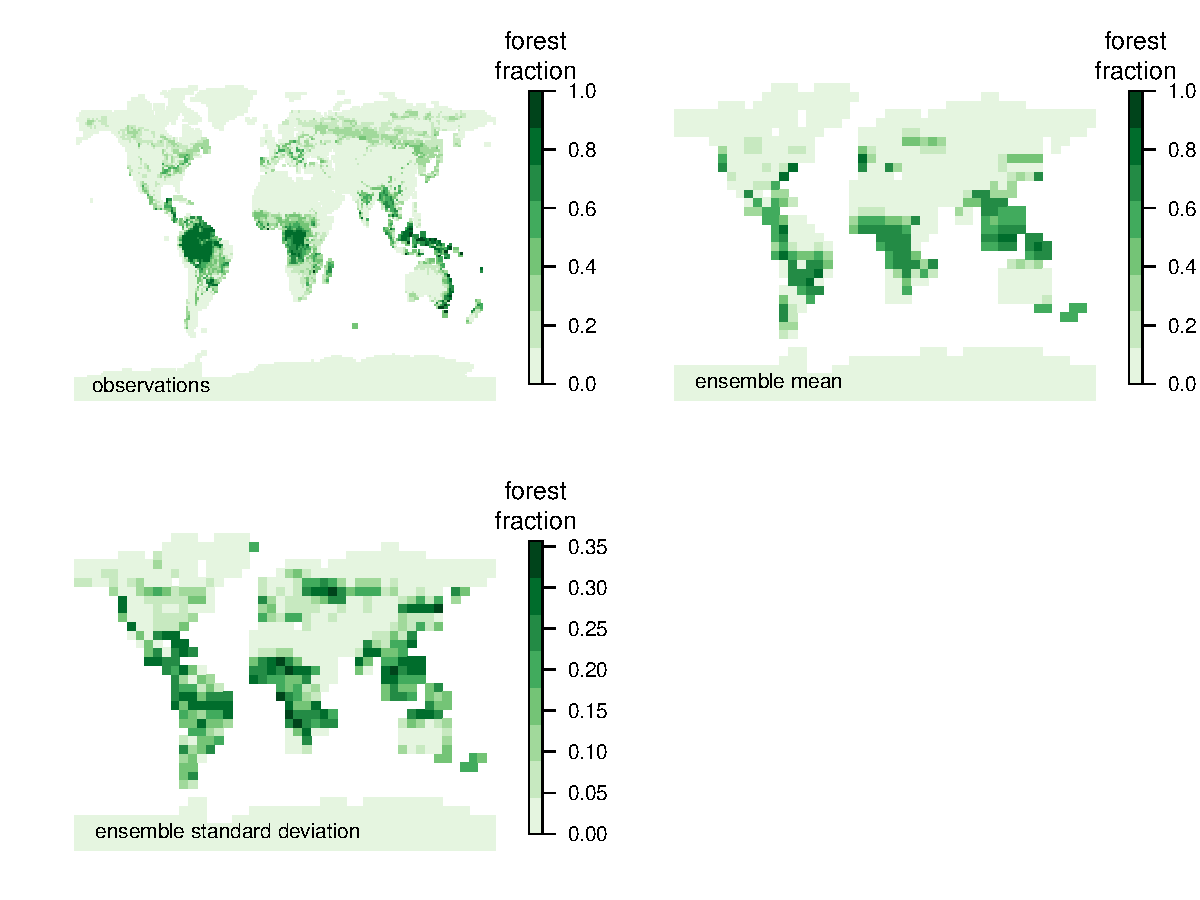
\includegraphics[width=12cm]{graphics/BL_obs_ensemble_mean_sd.pdf}
\caption{TEXT}
\label{fig:BL_obs_ensemble_mean_sd}
\end{figure}

\begin{figure}[t]
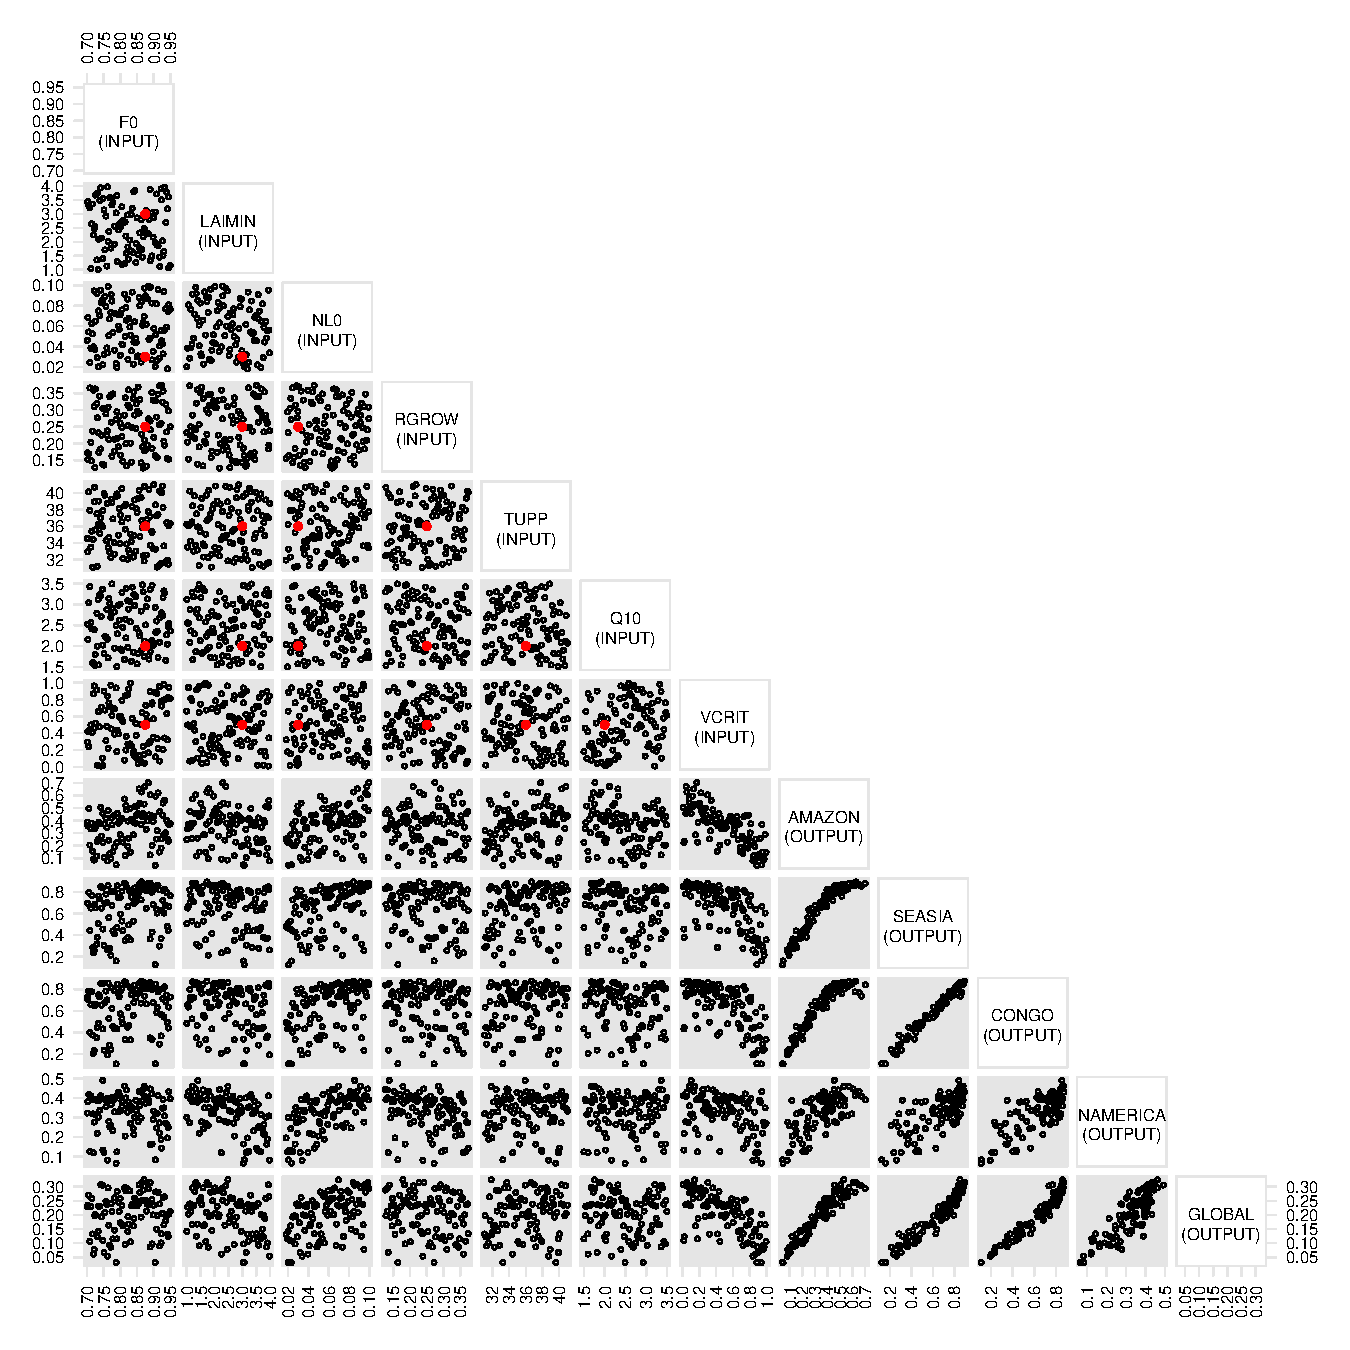
\includegraphics[width=12cm]{graphics/frac_pairs.pdf}
\caption{TEXT}
\label{fig:frac_pairs}
\end{figure}

\begin{figure}[t]
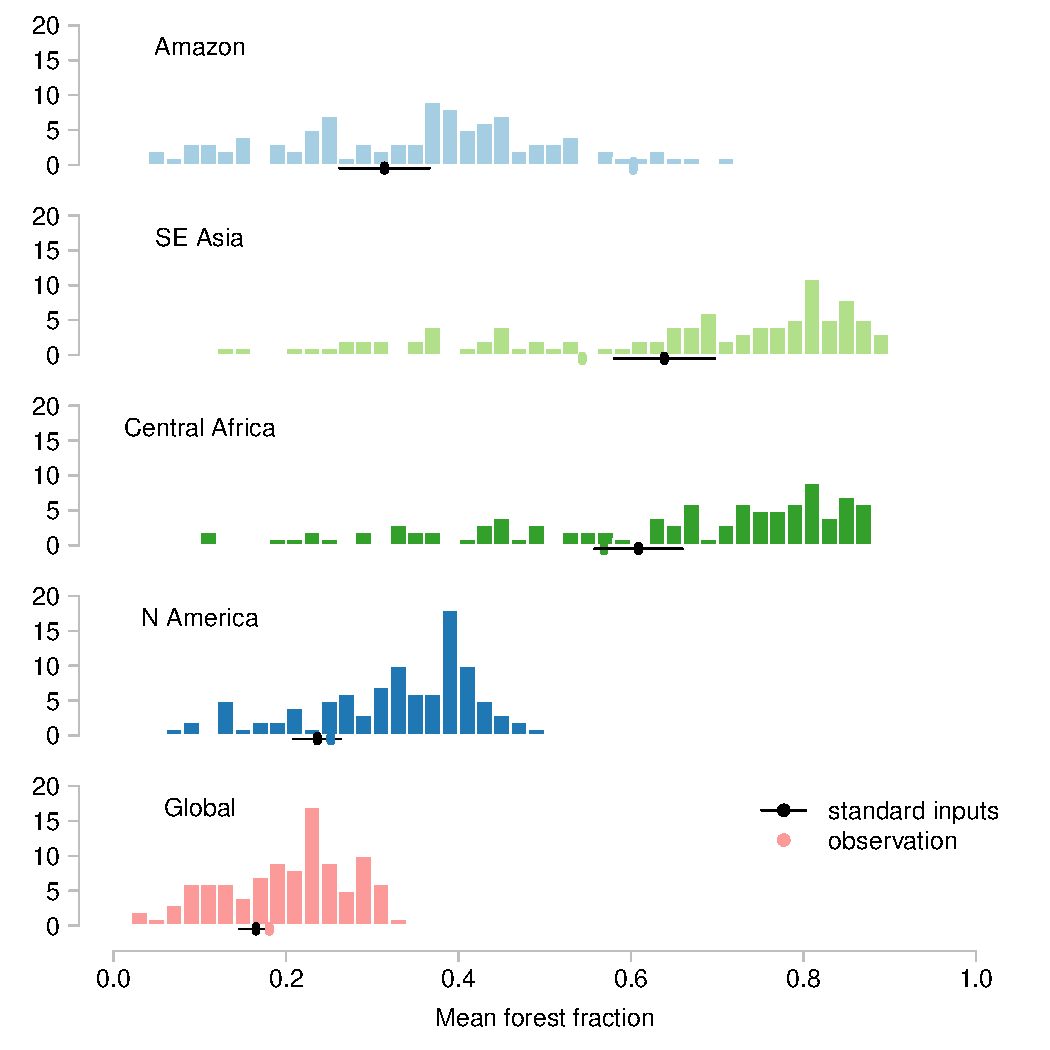
\includegraphics[width=12cm]{graphics/fraction_histogram_with_discrepancy_standard.pdf}
\caption{TEXT}
\label{fig:fraction_histogram_with_discrepancy_standard}
\end{figure}

\begin{figure}[t]
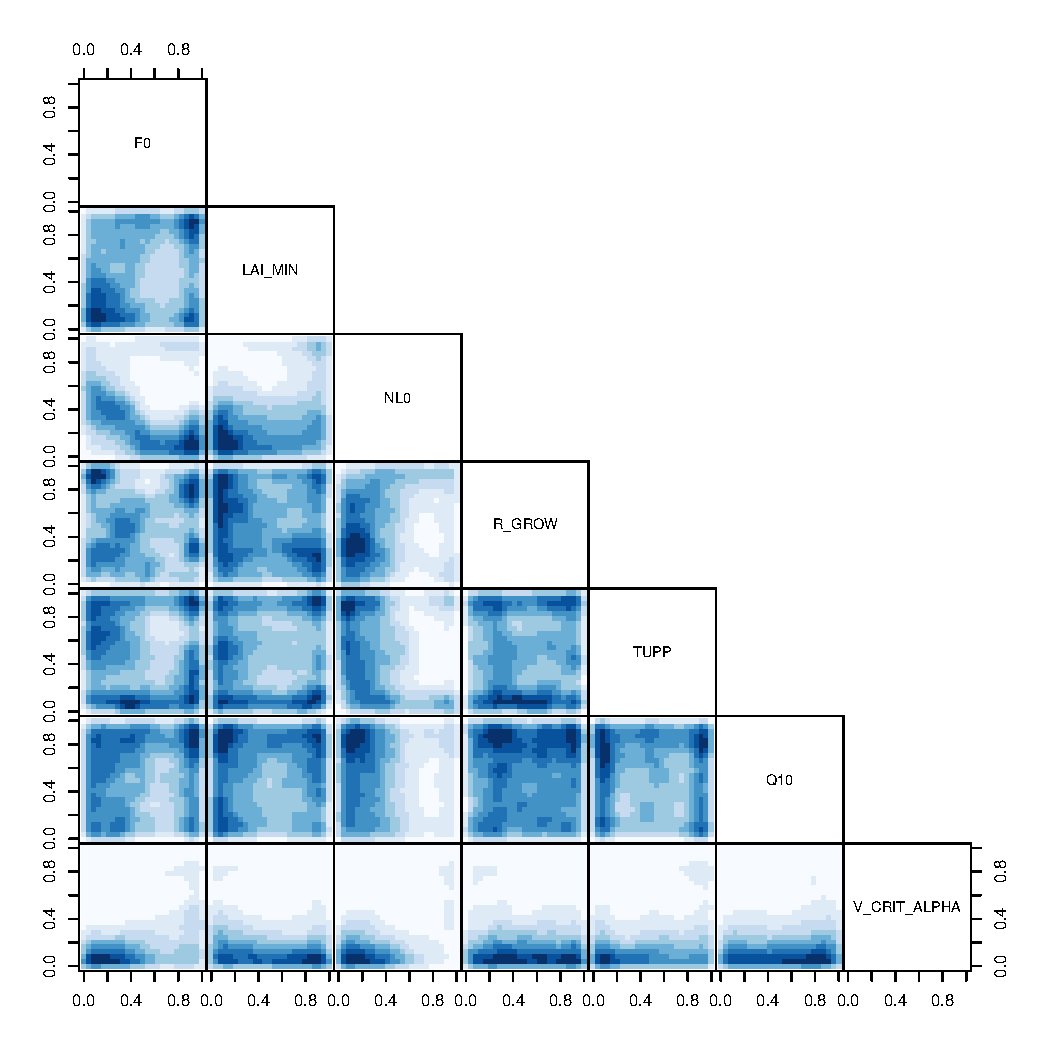
\includegraphics[width=12cm]{graphics/credible_NROY.pdf}
\caption{TEXT}
\label{fig:credible_NROY}
\end{figure}

\begin{figure}[t]
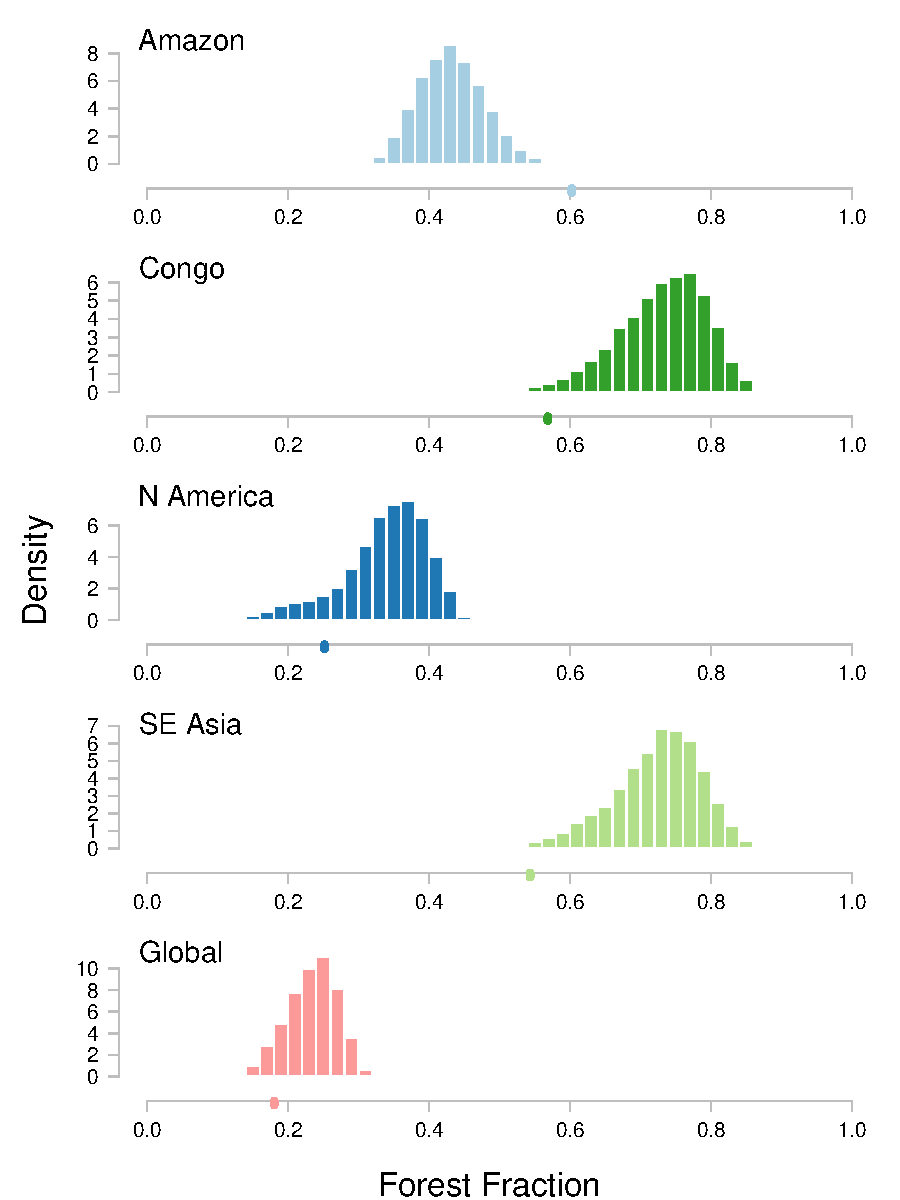
\includegraphics[width=12cm]{graphics/credible_NROY_hists.pdf}
\caption{TEXT}
\label{fig:credible_NROY_hists}
\end{figure}

\begin{figure}[t]
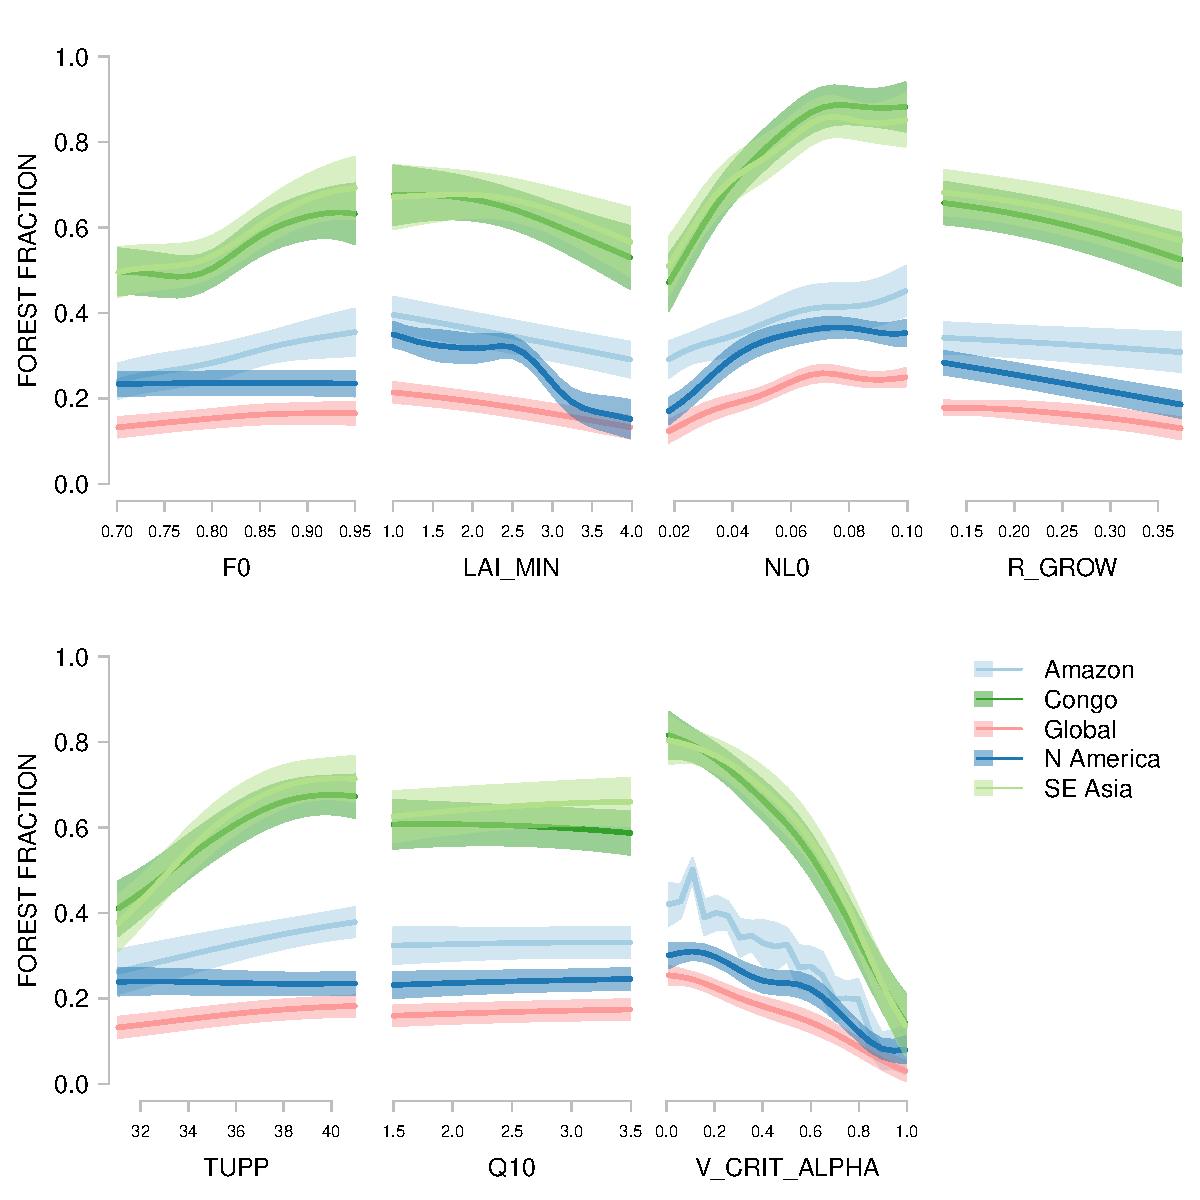
\includegraphics[width=12cm]{graphics/amaz_oat_sens.pdf}
\caption{TEXT}
\label{fig:amaz_oat_sens}
\end{figure}

\begin{figure}[t]
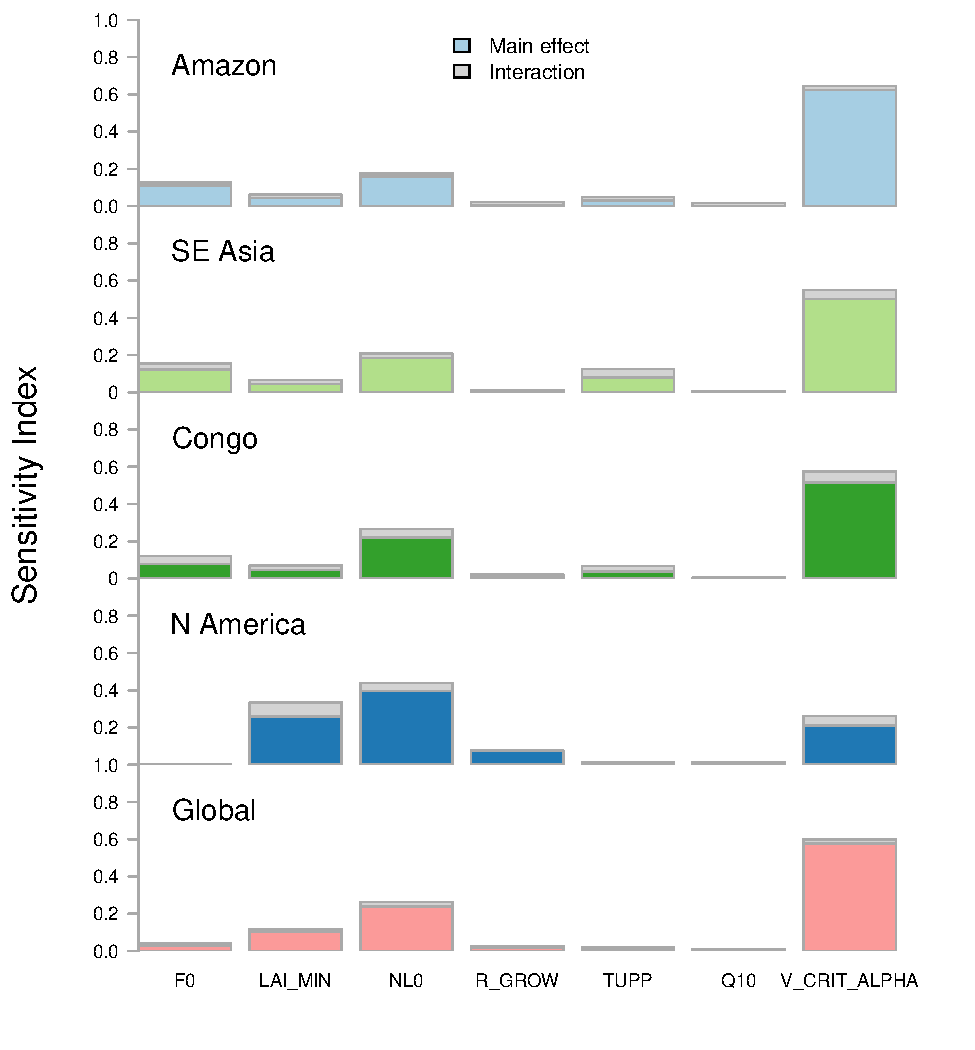
\includegraphics[width=12cm]{graphics/FAST_histograms.pdf}
\caption{TEXT}
\label{fig:FAST_histograms}
\end{figure}

\begin{figure}[t]
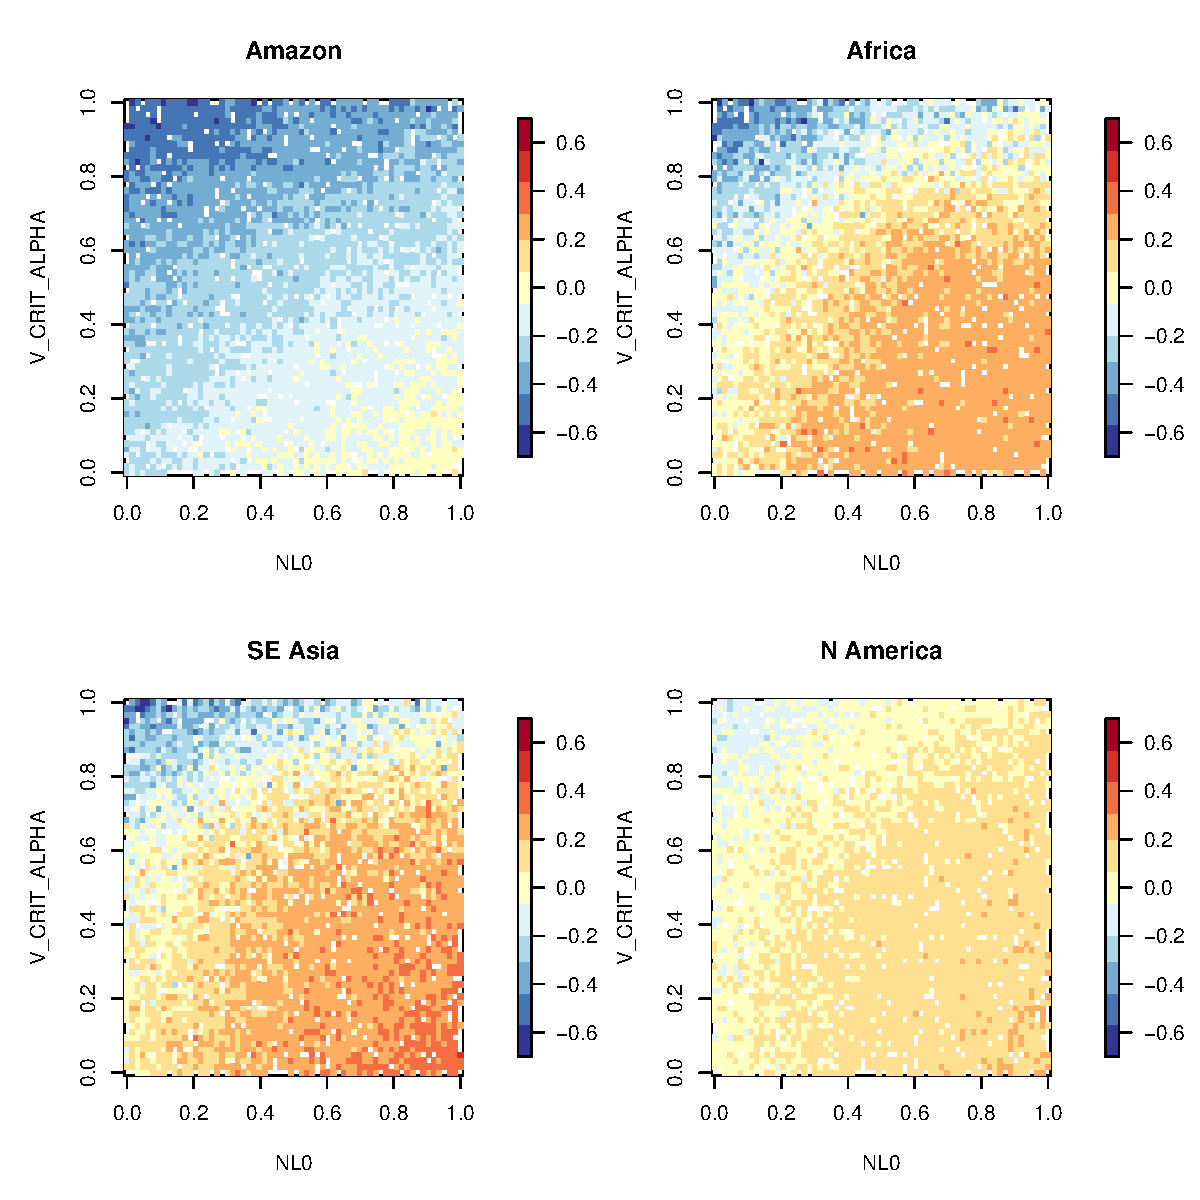
\includegraphics[width=12cm]{graphics/discrepancy_parameter_space.pdf}
\caption{TEXT}
\label{fig:discrepancy_parameter_space}
\end{figure}

\begin{figure}[t]
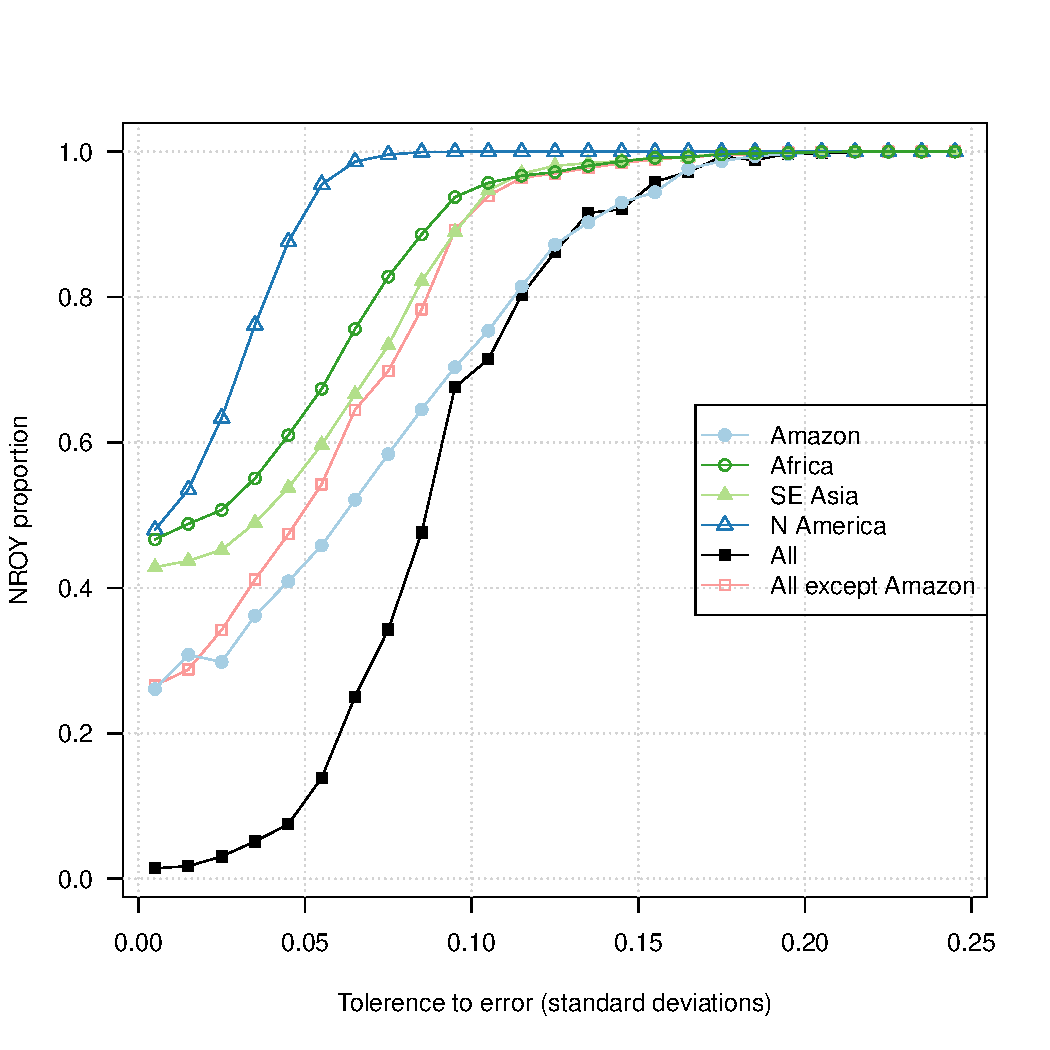
\includegraphics[width=12cm]{graphics/Prop_NROY_tolerance_unc.pdf}
\caption{TEXT}
\label{fig:Prop_NROY_tolerance_unc}
\end{figure}

\begin{figure}[t]
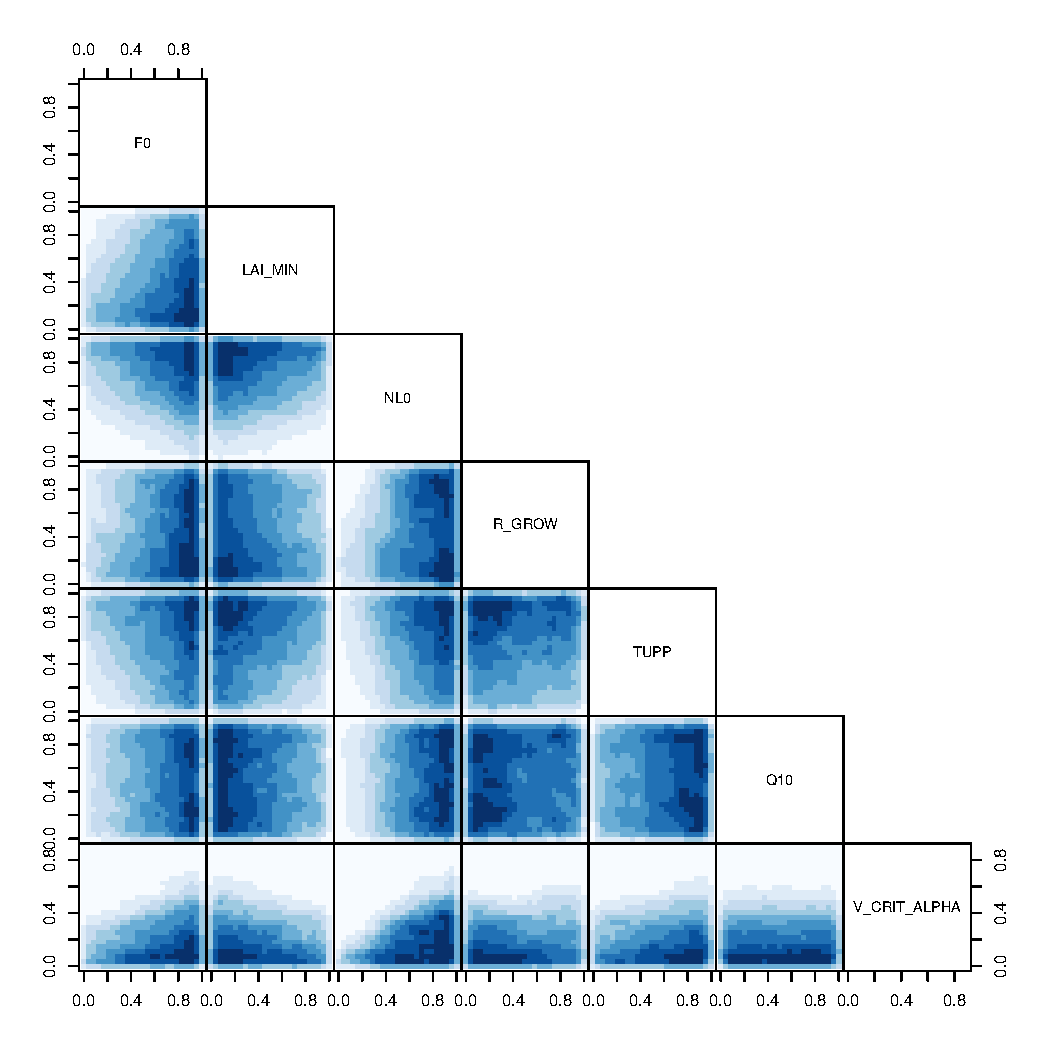
\includegraphics[width=12cm]{graphics/best_inputs_amazon.pdf}
\caption{TEXT}
\label{fig:best_inputs_amazon}
\end{figure}

\begin{figure}[t]
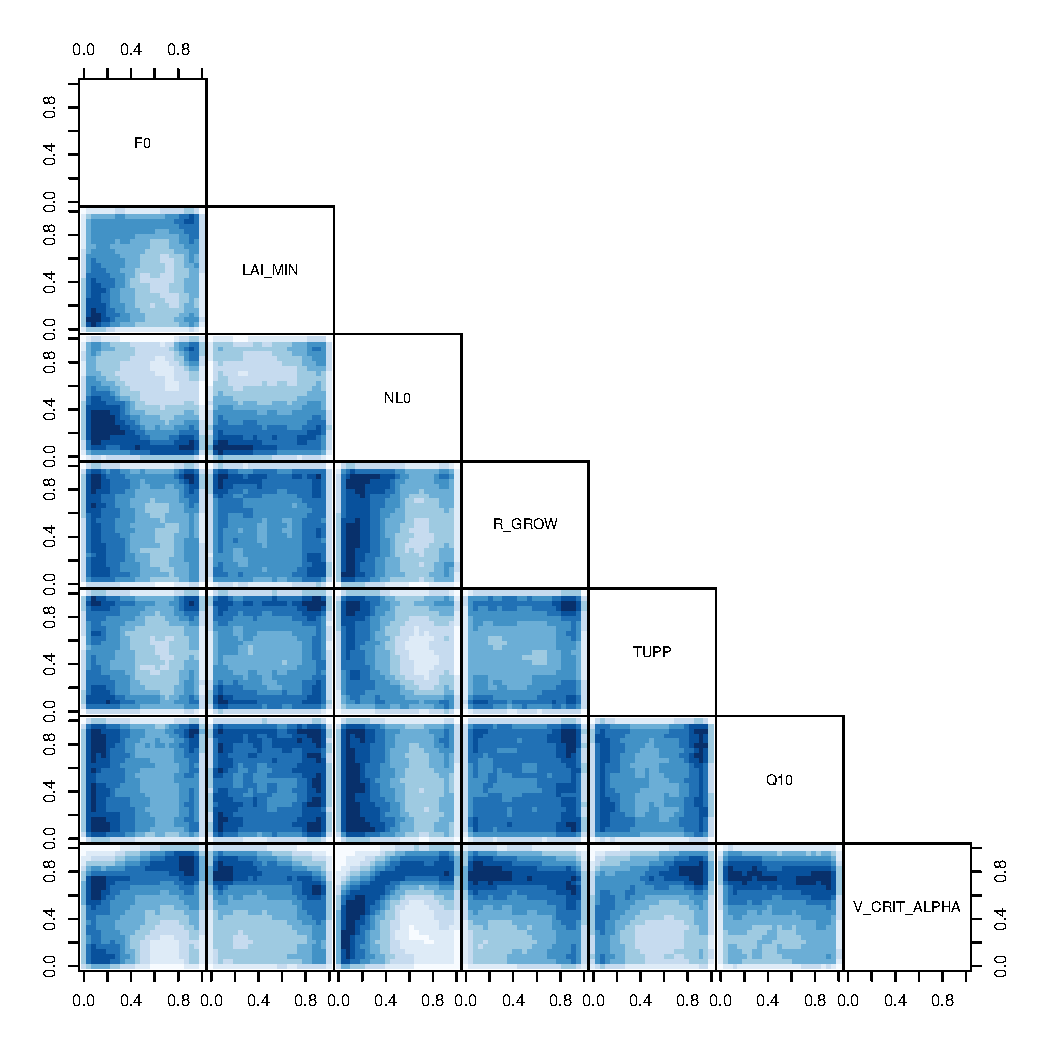
\includegraphics[width=12cm]{graphics/best_inputs_congo.pdf}
\caption{TEXT}
\label{fig:}
\end{figure}

\begin{figure}[t]
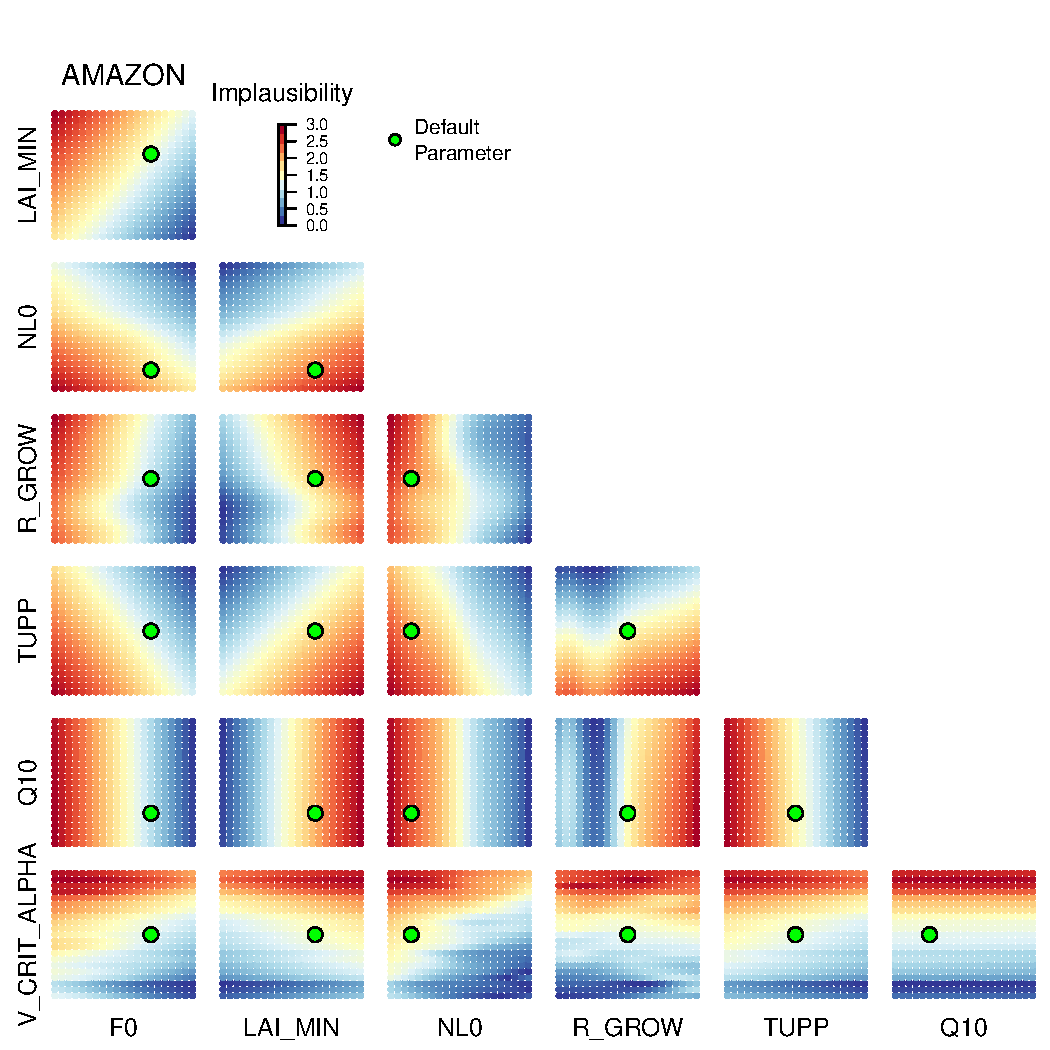
\includegraphics[width=12cm]{graphics/taat_amaz.pdf}
\caption{TEXT}
\label{fig:taat_amaz}
\end{figure}

\begin{figure}[t]
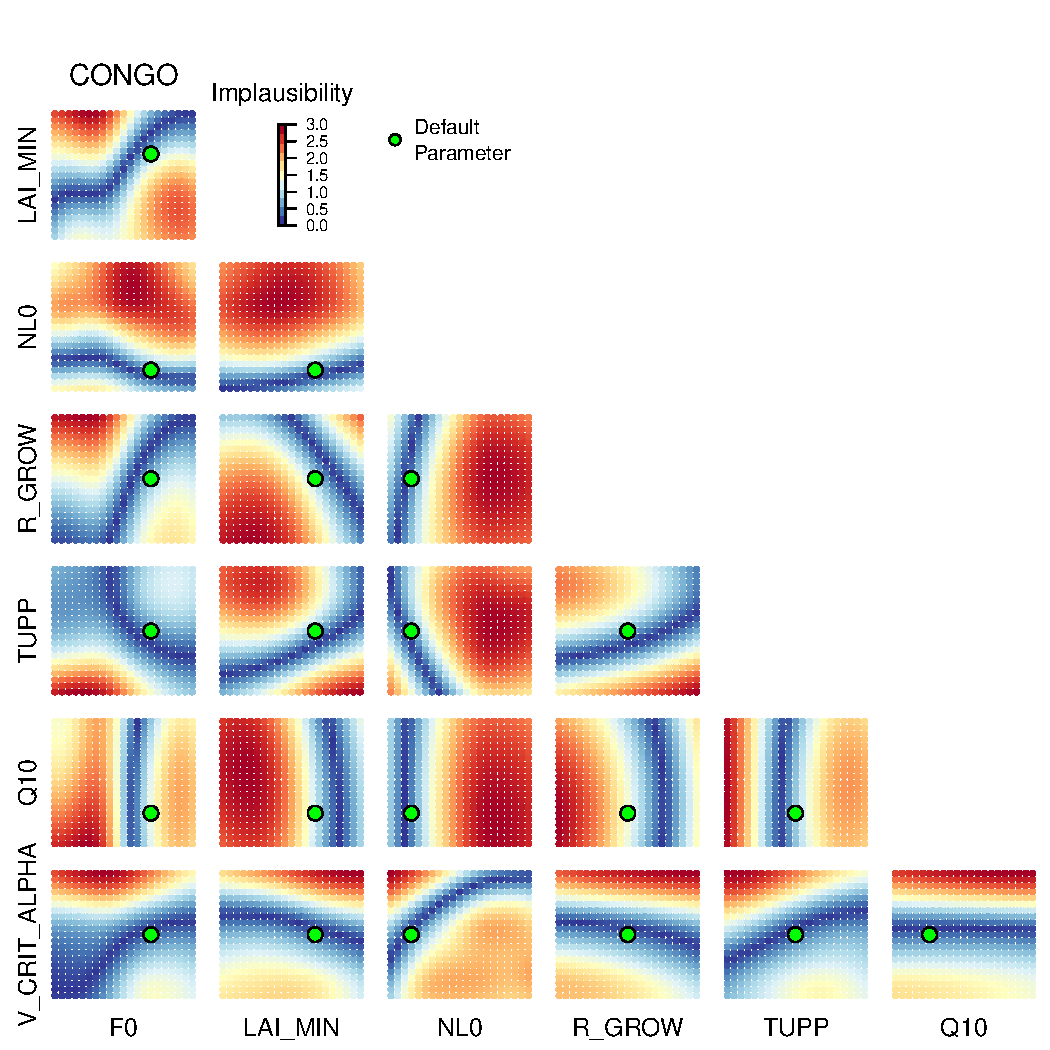
\includegraphics[width=12cm]{graphics/taat_congo.pdf}
\caption{TEXT}
\label{fig:}
\end{figure}

\begin{figure}[t]
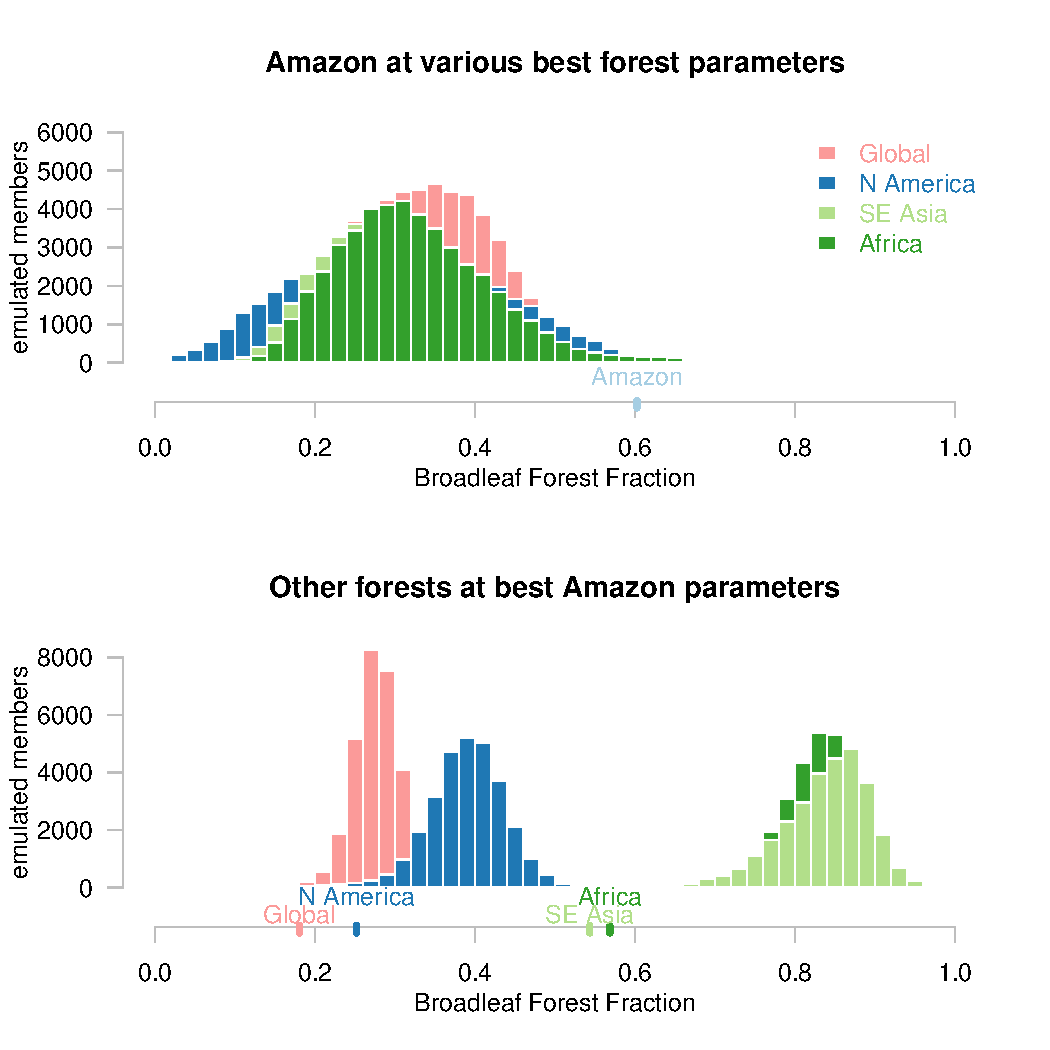
\includegraphics[width=12cm]{graphics/best_inputs_swaps_hists_Paired.pdf}
\caption{TEXT}
\label{fig:best_inputs_swaps_hists_Paired}
\end{figure}

\begin{figure}[t]
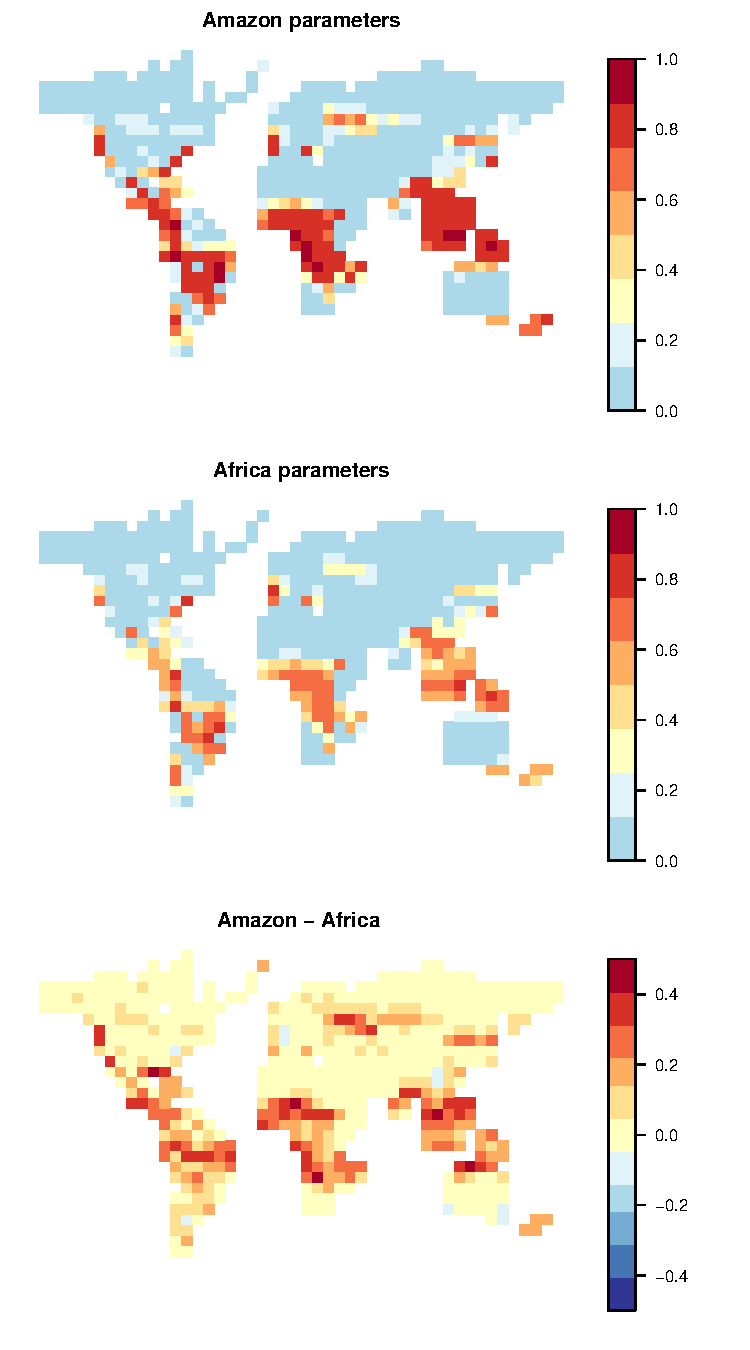
\includegraphics[width=8.3cm]{graphics/best_X_maps.pdf}
\caption{TEXT}
\label{fig:best_X_maps}
\end{figure}

\begin{figure}[t]
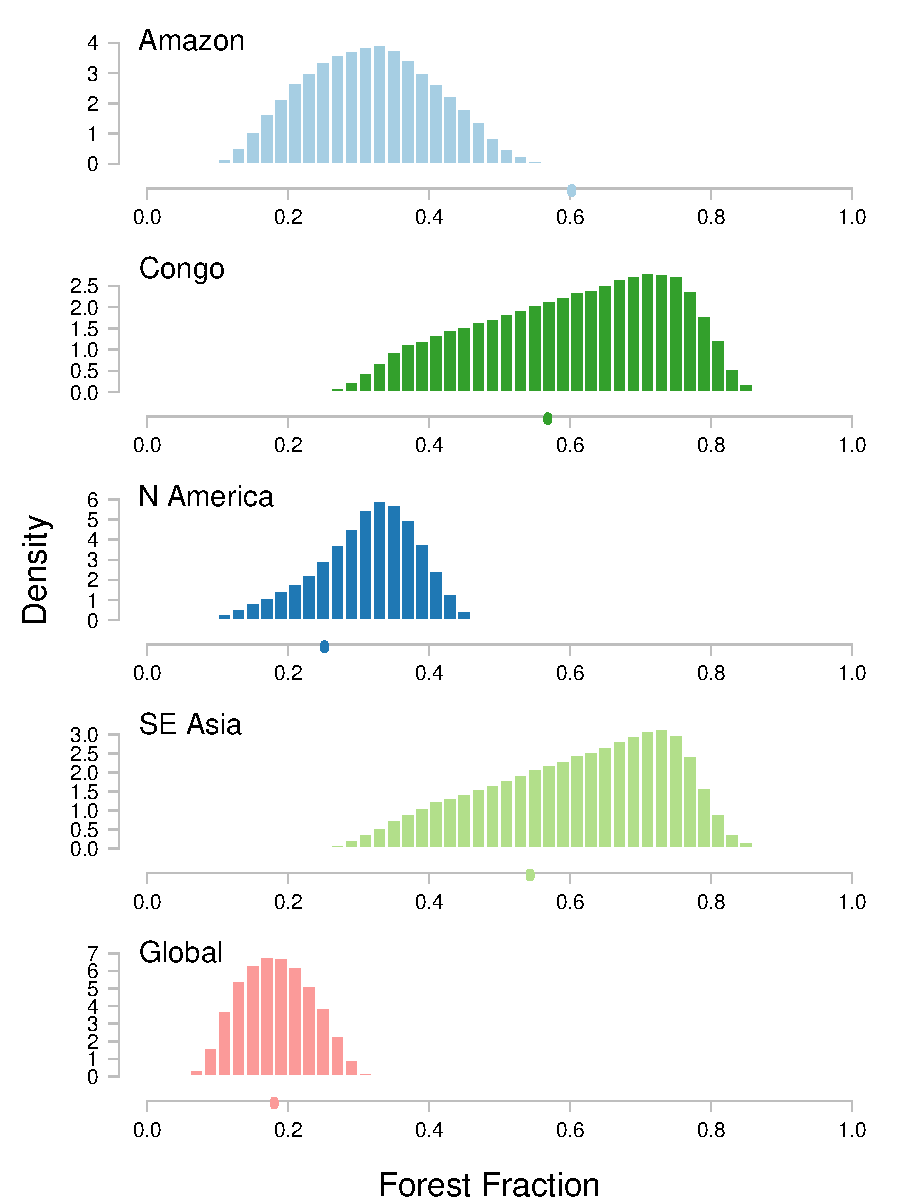
\includegraphics[width=12cm]{graphics/credible_NROY_hists_disc.pdf}
\caption{TEXT}
\label{fig:credible_NROY_hists_disc}
\end{figure}

\begin{figure}[t]
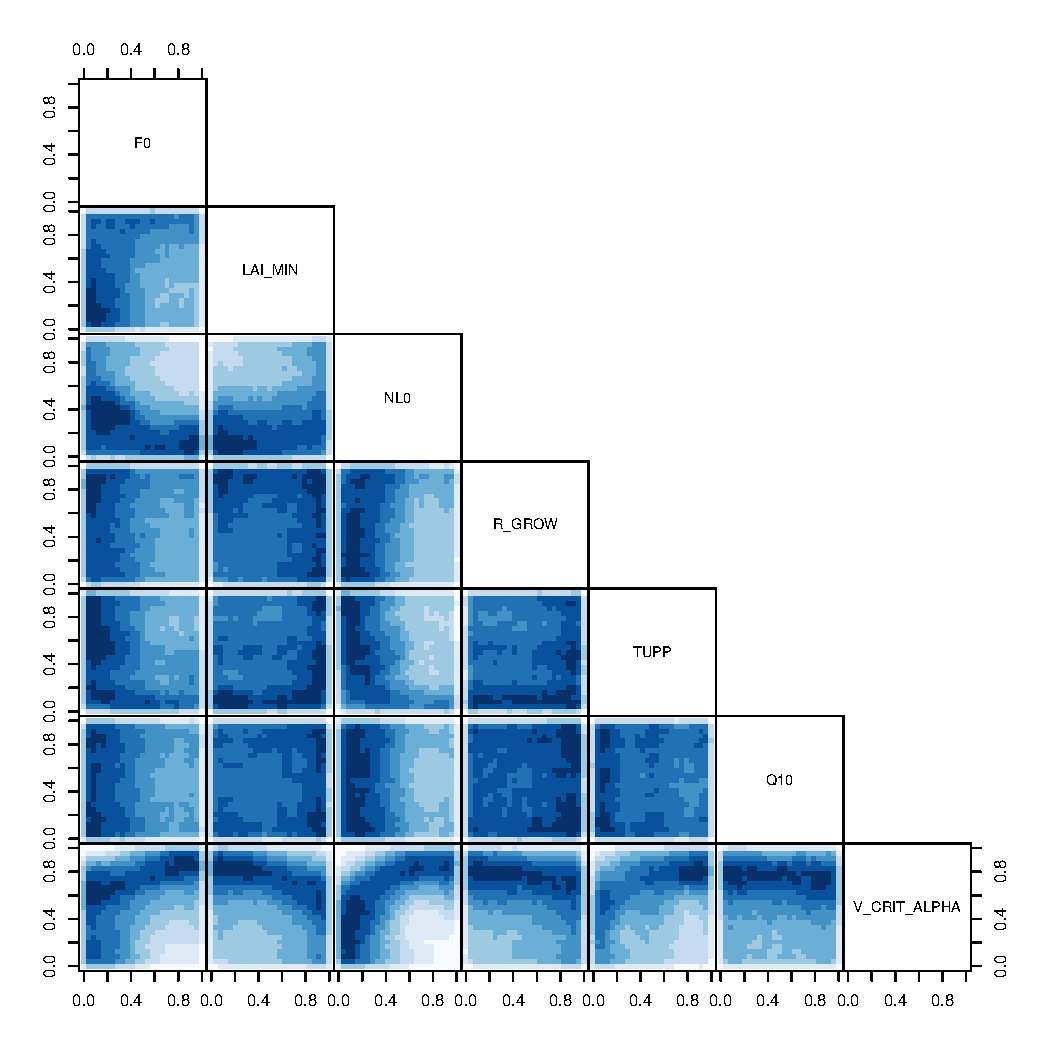
\includegraphics[width=12cm]{graphics/plausible_disc_input_space.pdf}
\caption{TEXT}
\label{fig:plausible_disc_input_space}
\end{figure}

\begin{figure}[t]
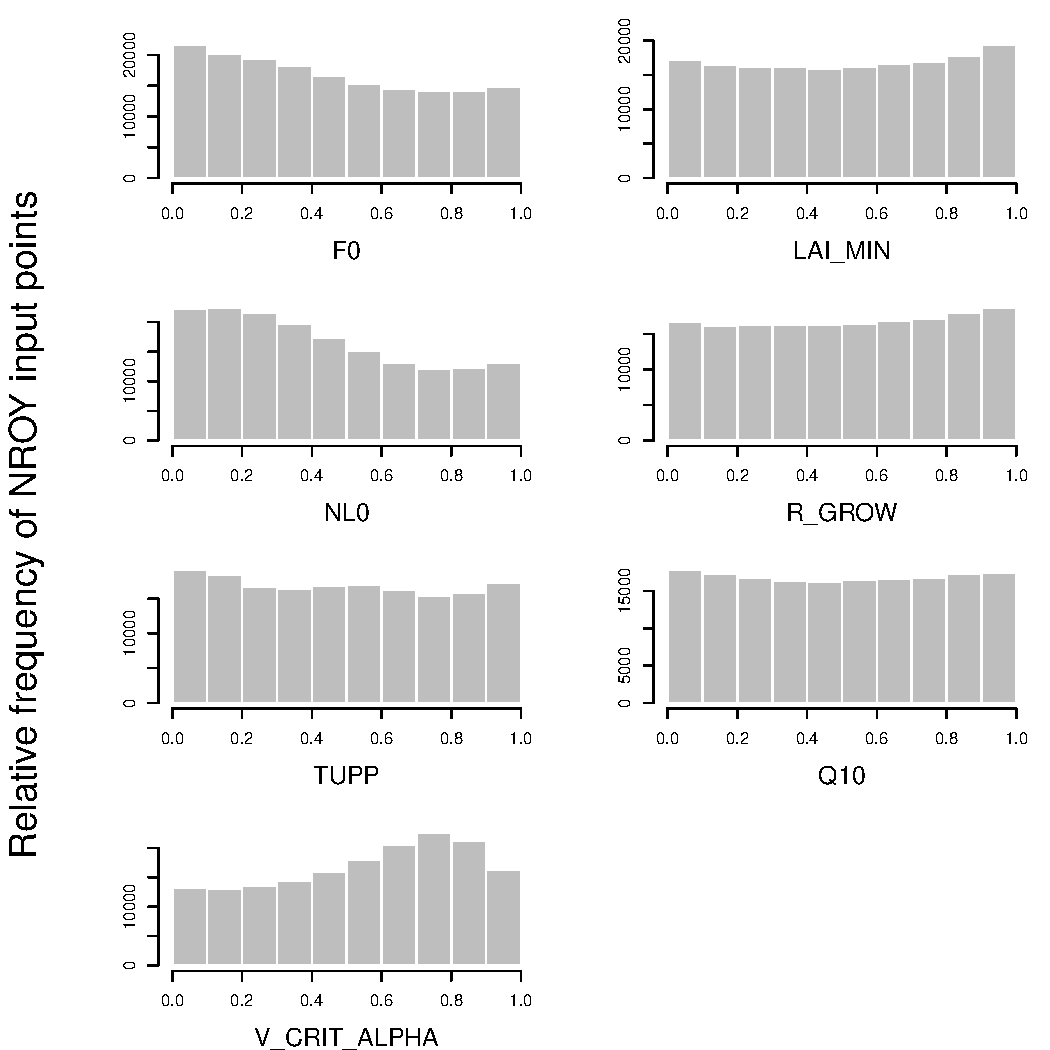
\includegraphics[width=12cm]{graphics/input_frequency_marginal.pdf}
\caption{TEXT}
\label{fig:input_frequency_marginal}
\end{figure}

%\begin{figure}[t]
%\includegraphics[width=12cm]{graphics/.pdf}
%\caption{TEXT}
%\label{fig:}
%\end{figure}



%% ONE-COLUMN FIGURES

%%f
%\begin{figure}[t]
%\includegraphics[width=8.3cm]{FILE NAME}
%\caption{TEXT}
%\end{figure}
%
%%% TWO-COLUMN FIGURES
%
%%f
%\begin{figure*}[t]
%\includegraphics[width=12cm]{FILE NAME}
%\caption{TEXT}
%\end{figure*}
%
%
%%% TABLES
%%%
%%% The different columns must be seperated with a & command and should
%%% end with \\ to identify the column brake.
%
%%% ONE-COLUMN TABLE
%
%%t
%\begin{table}[t]
%\caption{TEXT}
%\begin{tabular}{column = lcr}
%\tophline
%
%\middlehline
%
%\bottomhline
%\end{tabular}
%\belowtable{} % Table Footnotes
%\end{table}
%
%%% TWO-COLUMN TABLE
%
%%t
%\begin{table*}[t]
%\caption{TEXT}
%\begin{tabular}{column = lcr}
%\tophline
%
%\middlehline
%
%\bottomhline
%\end{tabular}
%\belowtable{} % Table Footnotes
%\end{table*}
%
%
%%% NUMBERING OF FIGURES AND TABLES
%%%
%%% If figures and tables must be numbered 1a, 1b, etc. the following command
%%% should be inserted before the begin{} command.
%
%\addtocounter{figure}{-1}\renewcommand{\thefigure}{\arabic{figure}a}
%
%
%%% MATHEMATICAL EXPRESSIONS
%
%%% All papers typeset by Copernicus Publications follow the math typesetting regulations
%%% given by the IUPAC Green Book (IUPAC: Quantities, Units and Symbols in Physical Chemistry,
%%% 2nd Edn., Blackwell Science, available at: http://old.iupac.org/publications/books/gbook/green_book_2ed.pdf, 1993).
%%%
%%% Physical quantities/variables are typeset in italic font (t for time, T for Temperature)
%%% Indices which are not defined are typeset in italic font (x, y, z, a, b, c)
%%% Items/objects which are defined are typeset in roman font (Car A, Car B)
%%% Descriptions/specifications which are defined by itself are typeset in roman font (abs, rel, ref, tot, net, ice)
%%% Abbreviations from 2 letters are typeset in roman font (RH, LAI)
%%% Vectors are identified in bold italic font using \vec{x}
%%% Matrices are identified in bold roman font
%%% Multiplication signs are typeset using the LaTeX commands \times (for vector products, grids, and exponential notations) or \cdot
%%% The character * should not be applied as mutliplication sign
%
%
%%% EQUATIONS
%
%%% Single-row equation
%
%\begin{equation}
%
%\end{equation}
%
%%% Multiline equation
%
%\begin{align}
%& 3 + 5 = 8\\
%& 3 + 5 = 8\\
%& 3 + 5 = 8
%\end{align}
%
%
%%% MATRICES
%
%\begin{matrix}
%x & y & z\\
%x & y & z\\
%x & y & z\\
%\end{matrix}
%
%
%%% ALGORITHM
%
%\begin{algorithm}
%\caption{�}
%\label{a1}
%\begin{algorithmic}
%�
%\end{algorithmic}
%\end{algorithm}
%
%
%%% CHEMICAL FORMULAS AND REACTIONS
%
%%% For formulas embedded in the text, please use \chem{}
%
%%% The reaction environment creates labels including the letter R, i.e. (R1), (R2), etc.
%
%\begin{reaction}
%%% \rightarrow should be used for normal (one-way) chemical reactions
%%% \rightleftharpoons should be used for equilibria
%%% \leftrightarrow should be used for resonance structures
%\end{reaction}
%
%
%%% PHYSICAL UNITS
%%%
%%% Please use \unit{} and apply the exponential notation


\end{document}
